\chapter{Introduction}
\section{Why Quantum Computation?}
% Add more chapters and sections related to Quantum Computing here
Quantum computers are the only model of computation that escape the limitations on computation imposed by the extended Church-Turing Thesis. These theoretical limitations will soon have practical consequences as Moore's Law (the doubling every eighteen months in transistor density on chips and the resulting increase in computer speed) is expected in a decade or so to run into inherent (classical) physical limits such as transistors scaling down to the size of elementary particles. 

Quantum computers would have a profound effect on complexity based cryptography, via the polynomial time quantum algorithms for factoring and discrete logs. Understanding how to meet these threats by designing quantum resistant crypto systems or by restoring to quantum cryptography is a major challenge.

Quantum computation has brought a renaissance in the examination of the foundations of quantum mechanics: highlighting phenomena such as entanglement and the resulting exponential power inherent in quantum physics, and showing that quantum error-correcting codes may be used to bring stability into the seemingly inherent unstable quantum world.

Lastly, the study of quantum computation has helped broaden and deepen our insights into complexity theory (and tools such as Fourier Analysis and information theory), and in a few cases helped resolve open questions in classical complexity theory.

Nature at the sub-atomic scale behaves totally differently from anything that our experience with the physical world prepares us for. Quantum mechanics is the name of the branch of physics that governs the world of elementary particles such as electrons and photons, and it is paradoxical, unintuitive, and radically strange. below is a sampling of a few such odd features.
\begin{itemize}
    \item Complete knowledge of as system's state is forbidden - A measurement reveals only a small amount of information about the quantum state of the system.
    \item The act of measuring a particle fundamentally disturbs its state.
    \item Quantum entities do not have trajectories. All that we can say for an elementary particle is that is started at A and was measured later at B. We cannot say anything about the trajectory or path it took from A to B.
    \item Quantum mechanics is inherently probabilistic. If we prepare two elementary particles in identical states and measure them, the result may be different for each particle.
    \item Quantum entities behave in some ways like particles and in others like waves. but they really behave in their own unique way, neither particles nor waves.
\end{itemize}
These features are truly strange, and difficult to accept. To quote the great physicist Niels Bohr, "Anyone who is not shocked by quantum theory has not understood it". We start by describing a simple experiment that highlights many differences between quantum mechanics and our classical intuition. It is the famous double slit experiment. The intuition gained in the process will help us define qubits, and more generally in the study of quantum computing.

This chapter introduces the basic framework of quantum information, including the description of quantum states as vectors with complex number entries, measurements that allow classical information to be extracted from quantum states, and operations on quantum states that are described by unitary matrices. We will restrict our attention in this chapter to the comparatively simple setting in which a single system is considered in isolation. We will then expand our view to multiple systems, which can interact with one another and be correlated, for instance.

There are, in fact, two common mathematical descriptions of quantum information. The one introduced in this lesson is the simpler of the two. This description is sufficient for understanding many (or perhaps most) quantum algorithms, and is a natural place to start from a pedagogical viewpoint.

A more general, and ultimately more powerful description of quantum information, in which quantum states are represented by density matrices, will be introduced in a later lesson. The density matrix description is essential to the study of quantum information, for several reasons. As examples, they can be used to model the effects of noise on quantum computations, or the state of one piece of an entangled pair. More generally, density matrices serve as a mathematical basis for quantum information theory and quantum cryptography, and are quite beautiful from a mathematical perspective. For these reasons, we encourage you to learn more about it when the time is right, but for now our focus will be on the simpler description of quantum information.
\section{The Double Slit Experiment}
What is the nature of light? You may have learned light is electromagnetic waves propagating through space. Also, you may have learned that light is made of a rain of individual particles called photon. but these two notions seem contradictory, how can it be both?

The debate over the nature of light goes deep into the history of science. The eminent physicist Isaac Newton believed that light was a rain of particles, called corpuscles. At the beginning of the nineteenth century, Thomas Young demonstrated with his famour double-slit interference experiment that light propagates as electromagnetic waves, and the debate seemed to be over. However, in 1905, Einstein was able to explain the photoelectric effect by using the idea of light quanta, or particles which we now call photons.

Similar confusion reigned over the nature of electrons, which behaved like particles, but then it was discovered in electron diffraction experiments, performed in 1927, that they exhibit wave behavior. So do the electrons behave like particles or waves? And what about photons? This great challenge was resolved with the discovery of the equations of quantum mechanics. but the theory is not intuitive, and its description of matter is very different from our common experience.

To understand what seems to be a paradox, we look to Young's double slit experiment. Here's the setup: a source of light is shone at a screen with two very thin, identical slits cut into it. Some light passes through the two slits and lands upon a subsequent screen. Take a look at the figure for a diagram of the experiment setup.

First, think what would happen to a stream of bullets going through this double slit experiment. The source, which we think of as a machine gun, is unsteady and sprays the bullets in the general direction of the two slits. Some bullets pass through one slit, some pass through the other slit, and others don't make it through one slits. The bullets that do go through the slits then land on the observing screen behind them. Now suppose we closed slit 2. Then the bullets can only go through slit 1 and land in a small spread behind slit 1. If we graphed the number of times a bullet that went through slit 1 and landed at the position y on the observation screen, we would see a normal distribution centered directly behind slit 1. That is, most land directly behind the slit, but some stray off a little due to the small amount randomness inherent in the gun, and because of they ricochet off the edges of the slit. If we now close slit 1 and open slit 2, we could see a normal distribution centered at slit 2.

Now let's repeat the experiment with bolt slits open. If we graph the number of times a bullet that went through either slit landed at the position y, we should see the sum of the graph we made for slit 1 and the graph for slit 2.

Another way we can thinks of the graphs we made is as graphs of the probability that a bullet will land at a particular spot on y on the screen. Let $P_1(y)$ denote the probability that the bullet lands at point y when only slit 1 is open, and similarly for $P_2(y)$. And let $P_{12}(y)$ denote the probability that the bullet lands at point y when both slits are open. Then $P_{12}(y)=P_1(y)+P_2(y)$.

\begin{figure}
    \centering
    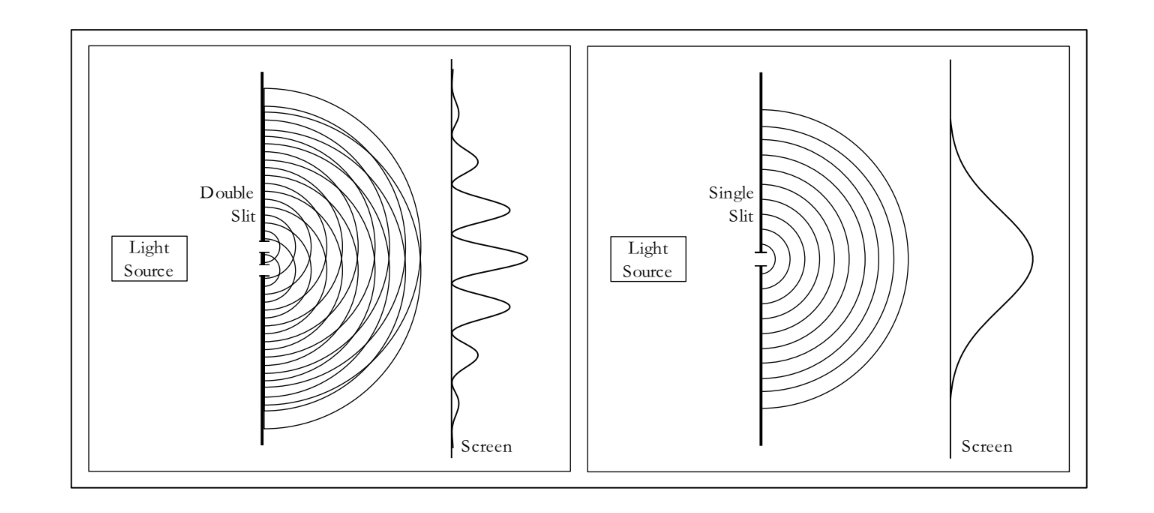
\includegraphics[width=1\linewidth]{Images/Doubleslit.png}
    \caption{Double slit and single-slit diffraction}
    \label{fig:slitexperiment}
\end{figure}

Next, we consider the situation for waves, for example water waves. A water wave doesn't go through either slit 1 or slit 2, it goes through both. you should imagine the rest of 1 water wave as it approaches the slit. As it hits the slit, the wave is blocked at all places but the two slits, and waves on the other side are generated at each slit as depicted in the figure \ref{fig:slitexperiment}.

When the new waves generated at each slit run into each other, interference occurs. We can see this by plotting the intensity (that is, the amount of energy carried by the waves) at each point y along the viewing screen. What we see is the familiar interference pattern seen in figure \ref{fig:slitexperiment}. The dark patches of the interference pattern seen in figure \ref{fig:slitexperiment} occur where the wave from the first slit arrives perfectly out of sync with wave from the second slit, while the bright points are where the two arrive in sync. For example, the bright spot right in the middle is bright because each wave travels the exact same distance from their respective slits to the screen, so they arrive in sync. The first dark spots are where the wave from one slit traveled exactly half of a wavelength longer than the other wave, thus they arrive at opposite points in their cycle and cancel. Here, it is not the intensities coming from each slit that add, but the height of the wave. This differs in the case of bullets: $I_{12}(y)\neq I_1(y)+I_2(y)$, but $h_{12}(y)=h_1(y)+h_2(y)$, and $I_{12}(y)=h(y)^2$, where $h9y)$ is the height of the wave and $I(y)$ is the intensity, or energy, of the wave.

Before we can say what light does, we need one more crucial piece of information. What happens when we turn down the intensity in both of these examples?

In the case of bullets, turning down the intensity means turning down the rate at which the bullets are fired. When we turn down the intensity, each time a bullet hits the screen it transfers the same amount of energy, but the frequency at which bullets hit the screen becomes less.

With water waves, turning down the intensity means making the wave amplitudes smaller. Each time a wave hits the screen it transfer less energy, but the frequency of the waves hitting the screen is unchanged.

Now what happens when we do this experiment with light. As Young observed in 1802, light makes an interference pattern on the screen. From this observation he concluded that the nature of light is wavelike, and reasonably so!.  However, Young was unable at the time to turn down the intensity of light to see the problem with the wave explanation.

Picture now that the observation screen is made of thousands of tiny little photo-detectors that can detect the energy they absorb. For high intensities the photo-detectors individually are picking up a lot of energy, and when we plot the intensity against the position y along the screen we see the same interference pattern as described earlier. Now, turn the intensity of the light very very low. At first, the intensity scales down lower and lower everywhere, just like a wave. But as soon as we get low enough, the energy that the photo-detectors report reaches a minimum energy, and all of the detectors are reporting the same energy, call it $E_0$, just at different rates. This energy corresponds to the energy carried by an individual photon, and at this stage we see what is called quantization of light. Photo-detectors that are in the bright spots of the interference pattern report the energy $E_0$ very frequently, while the darker areas report the energy $E_0$ at lower rates. Totally dark points still report nothing. This behavior is the behavior of bullets not waves! We now see that photons behave unlike either bullets or waves, but like something entirely different.

Turn down, the intensity so low that only one photo-detector reports something each second. in other words, the source only sends one photon at at time. Each time a detector receives a photon, we record where on the array it landed and plot it on a graph. The distribution we draw will reflect the probability that a single photon will land at a particular point.

Logically we think that the photon will either go through one slit or the other. Then, like the bullets, the probability that the photon lands at a point y should be $P_{12}(y)=P_1(y)+P_2(y)$ and the distribution we expect to see is the two peaked distribution of the bullets. But this is not what we see at all.

What we actually see is the same interference pattern as before! But how can this be? For there to be an interference pattern, light coming from one slit must interfere with light from the other slit; but there is only one photon going through at a time! The modern explanation is that the photon actually goes through both the slits at the same time, and interferes with itself. The mathematics is analogous to that in the case of water waves. We say that the probability $P(y)$ that a photon is detected at $y$ is proportional to the square of some quantity $a(y)$, which we call a probability amplitude. Now probability amplitudes for different alternatives add up. So $a_{12}(y)=a_{1}(y)+a_2(y)$. But $P_{12}(y)=|a_{12}(y)|^2\neq |a_1(y)|^2+|a_2(y)|^2=P_1(y)+P_2(y)$.

Logically, we can ask which slit the photon went through, and try to measure it. Thus, we might construct a double slit experiment where we put a photo-detector at each slit, so that each time a photon comes through the experiment we see which slit it went through and where it hits on the screen. but when such an experiment is performed, the interference pattern gets completely washed out! The very fact that we know which slit the photon goes through makes the interference pattern go away. This is the first example we see of how measuring a quantum system alters the system.

Here the photon looks both like a particle, a discreet package , and a wave that can have interference. It seems that the photon acts like both a wave and a particle, but at the same time it doesn't exactly behave like either. This is what is commonly known as the wave-particle duality, usually though of as a paradox. The resolutions is that the quantum mechanical behavior of matter is unique, something entirely new.

What may be more mind blowing still is that if we conduct the exact same experiment with electrons instead of light, we get the exact same results! Although it is common to imagine electrons as tiny little charged spheres, they are actually quantum entities, neither wave nor particle but understood by their wave function.

The truth is that there is no paradox, just an absence of intuition for quantum entities. Why should they be intuitive? Things on our scale do not behave like wave functions, and unless we conduct wild experiments like this we do not see the effects of quantum mechanics.
``  
\section{The Coin Experiment: Analogy for intuition}
Consider an unbiased coin, a preliminary high school knowledge will tell you that if you toss a coin the probability of getting heads or tails either is $1/2$. Given a coin we can either toss it or look at the coin. Note that we don't know the side of the coin facing up unless and until we look at the coin. This action of looking at the coin let us call it as measurement. Thus, given a coin we can perform two operations, either measurement or toss a coin i.e. we can either see the side facing up or toss the coin. Let us now move on to the mathematical framework. Consider that we don't know the state of the coin initially, so it can be either heads or tails with equal probability of $1/2$ and hence can be written as
\[
\begin{pmatrix} 1/2 \\ 1/2 \end{pmatrix}
\]
where the entry in the first row corresponds to the probability of seeing heads ($=1/2$) and the entry in the second row corresponds to seeing tails ($=1/2$) upon measurement. Note that the sum of the entries in the column must be equal to 1. Now we can either look at the coin i.e. do a measurement or toss a coin. Let us toss the coin. Now since it's an unbiased coin the state of the vector will not change even after tossing the coin. Mathematically, this can be represented by a linear operation i.e. matrix-vector multiplication operation where the matrix corresponds to the operation of tossing the coin. This is shown as follows:
\[
\begin{pmatrix} 1/2 & 1/2 \\ 1/2 & 1/2 \end{pmatrix} \begin{pmatrix} 1/2 \\ 1/2 \end{pmatrix} = \begin{pmatrix} 1/2 \\ 1/2 \end{pmatrix}
\]
where the matrix corresponds to the operation of tossing a coin and the vector is the state vector of the coin before tossing the coin. The state vector indicates that the probability of measuring heads is $1/2$ and probability measuring tails is $1/2$ upon measurement. Now if we perform a measurement i.e. look at the coin the probabilistic state of the coin it will either collapse to the following
\[
\begin{pmatrix} 1 \\ 0 \end{pmatrix} or \begin{pmatrix} 0 \\ 1 \end{pmatrix} 
\]
 for heads and tails respectively. Let us call this as basis states. Thus, if we perform another measurement the next time we will get Heads with certainty or tails with certainty depending upon the results of the previous measurement as indicated by the state vector which is also consistent with the real world results. Thus, we have a working mathematical framework of tossing a coin. Suppose, upon measurement we had found that the result of the state was head and hence the state vector was $\begin{pmatrix} 1 \\ 0 \end{pmatrix}$. Now when we toss the coin, we get
 \[
 \begin{pmatrix} 1/2 & 1/2 \\ 1/2 & 1/2 \end{pmatrix} \begin{pmatrix} 1 \\ 0 \end{pmatrix} = \begin{pmatrix} 1/2 \\ 1/2 \end{pmatrix}
 \]
 which is as we expected that now upon measurement the probability of getting heads is equal to the probability of getting tails $(=1/2)$. All the mathematical framework is consistent with the real world experiences. Now, no matter how many times we toss the coin the state of the vector will remain the same i.e. probability of getting heads is equal to the probability of getting tails $=1/2$ unless and until we perform a measurement by looking at the coin whereupon it collapses to one of the basis states.
Note that the state vector is also the eigen vector corresponding to the eigen value of 1 of the matrix (operation matrix of tossing the coin).

Let us make it more interesting by taking a biased coin. Let the probability of getting heads be 1/4 and of getting tails be 3/4. Thus the state vector corresponding to it will be
\[
\begin{pmatrix} 1/4 \\ 3/4 \end{pmatrix}
\]
We can now perform a measurement or toss the coin. Consider we don't know the state initially and we toss the coin, then the matrix-vector linear operation corresponding to the operation of tossing the coin and the state vector will be
\[
\begin{pmatrix} 1/4 & 1/4 \\ 3/4 & 3/4 \end{pmatrix}\begin{pmatrix} 1/4 \\ 3/4 \end{pmatrix} = \begin{pmatrix} 1/4 \\ 3/4 \end{pmatrix}
\]
Thus indicates that upon measurement we will get heads with a probability of $1/4$ and tails with a probability of $3/4$. No matter how many times we toss the coin the state of the vector will remain the same. Upon measurement the state will collapse to one of the basis states
\[
\begin{pmatrix} 1 \\ 0 \end{pmatrix} or \begin{pmatrix} 0 \\1 \end{pmatrix}
\]
Say upon measurement we found that it was Tails i.e. the state vector collapsed to $\begin{pmatrix} 0 \\1\end{pmatrix}$. Then again upon tossing the coin the state vector again be in a probabilistic state as follows:
\[
\begin{pmatrix} 1/4 & 1/4 \\3/4 & 3/4 \end{pmatrix} \begin{pmatrix} 0 \\ 1 \end{pmatrix} = \begin{pmatrix} 1/4 \\ 3/4\end{pmatrix}
\]
as expected. The state of the coin after tossing will again be a probabilistic state will the probability of getting heads being $1/4$ and the probability of tails being $3/4$ upon measurement.

Now, let us take this a step further. Note that we can write $\begin{pmatrix} 1/4 \\ 3/4 \end{pmatrix} = 1/4 \begin{pmatrix} 1 \\ 0 \end{pmatrix} + 3/4 \begin{pmatrix} 0 \\1\end{pmatrix}$. Note that we can write the state vector of the coin at any intermediate state as a linear combination of the basis state (since the basis states are two linearly independent orthogonal vectors, they span the entire 2D Vector space and hence any vector in the 2D space can be written as a linear combination of these two vectors). Thus, we can write the state vector of coin at any time as the linear combination of the basis states as shown below:
\[
\begin{pmatrix} \alpha \\ \beta \end{pmatrix} = \alpha \begin{pmatrix} 1 \\ 0 \end{pmatrix} + \beta \begin{pmatrix} 0 \\ 1 \end{pmatrix}
\]
for $\alpha, \beta \in \mathbb{R}$. Thus, the state vector of the coin always exists as a linear combination of the basis states. The operation of tossing the coin is simply a matrix-vector multiplication with the state as follows.
\begin{align*}
\begin{pmatrix} 1/4 & 1/4 \\3/4 & 3/4 \end{pmatrix} \begin{pmatrix} \alpha \\ \beta \end{pmatrix} &= \alpha \begin{pmatrix} 1/4 & 1/4 \\3/4 & 3/4 \end{pmatrix} \begin{pmatrix} 1 \\ 0 \end{pmatrix} + \beta \begin{pmatrix} 1/4 & 1/4 \\3/4 & 3/4 \end{pmatrix} \begin{pmatrix} 0 \\ 1 \end{pmatrix}\\
&= \alpha \begin{pmatrix} 1/4 \\ 3/4 \end{pmatrix} + \beta \begin{pmatrix} 1/4 \\ 3/4 \end{pmatrix}\\
&=(\alpha + \beta) \begin{pmatrix} 1/4 \\ 3/4 \end{pmatrix}
\end{align*}
Note that if we perform a measurement just after another measurement then the state of the vector remains unchanged i.e. say upon measurement we saw that the state vector was Heads then if we perform another measurement operation just after the first one (i.e. without tossing the coin) then the state vector will not change and will remain as Heads. No matter the amount of time you perform consecutive measurements the state vector once collapsed to either of the basis state in the first measurement remains the same throughout. But if we perform a matrix operation (coin toss) it will then again be in a probabilistic (or linear combination sometimes called a superposition) state.

In conclusion, we saw that the state vector is a linear combination of the basis vector (with real coefficients) and there are two categories of operations we can perform on the coin either measurement or toss a coin. Similar is the case with qubits. This linear combination of basis states is what sometimes referred to as the superposition principle.

For a qubit, the state vector is a linear combination (also called superposition) of the basis states (or vectors) (with complex coefficients) and there are two types of operations we can perform on qubits either measurement (in which case it collapses to one of the basis states) or a matrix multiplication (here the matrix is unitary as a result of Axiom of Quantum mechanics we will later see). Thus, we can define the basis vectors/states for the purpose of quantum computing as follows:
\[
\ket{0}=\begin{pmatrix} 1 \\ 0 \end{pmatrix}, \ket{1}=\begin{pmatrix} 0 \\ 1 \end{pmatrix}
\]
and thus the state vector of a qubit is given as
\[
\ket{v}=\begin{pmatrix} \alpha \\ \beta \end{pmatrix} = \alpha \begin{pmatrix} 1 \\ 0 \end{pmatrix} + \beta \begin{pmatrix} 0 \\ 1 \end{pmatrix}
\]
where $\alpha,\beta \in \mathbb{C}$. Thus, we can perform either of the two operations measurement or a matrix operation (manipulation of qubits). Upon measurement it will either collapse to either one of the basis states. The condition for manipulation of a matrix by a qubit is that it must be unitary. Thus, matrix multiplication will be as follows:
\[
Uv=\begin{pmatrix} a & b \\ c & d \end{pmatrix}\begin{pmatrix} \alpha \\ \beta \end{pmatrix} =\begin{pmatrix} a \alpha + b\beta \\ c\alpha + d\beta \end{pmatrix}
\]
where U is a unitary matrix ($U^{\dagger}U=UU^{\dagger}=I$).
There is another restriction that the norm of the state vector must be unit norm ($\|\ket{v}\|=1$). All these restrictions will be further explained in depth as part of axioms of Quantum Mechanics.

\section{Quantum Information}
We will look at Quantum information, a concept on which quantum computation is based.

\subsection{The Classical Information}
To describe quantum information and how it works, we will begin with an overview of classical information. Some readers may wonder why we choose to devote so much attention to classical information in a course on quantum information, but there are good reasons. For one, although quantum and classical information are different in some pretty spectacular ways, their mathematical descriptions are actually quite similar.

Classical information also serves as a familiar point of reference when studying quantum information, as well as a source of analogy that goes a surprisingly long way. It is common that people ask questions about quantum information that have natural classical analogs — often with simple answers that can provide both clarity and insight into the original questions about quantum information. Indeed, it is not at all unreasonable to claim that one cannot truly understand quantum information without understanding classical information.

Some readers may already be familiar with the material to be discussed in this section, while others may not — but the discussion is meant for both audiences. In addition to highlighting the aspects of classical information that are most relevant to an introduction to quantum information, this section introduces the Dirac notation, which is often used to describe vectors and matrices in quantum information and computation. As it turns out, the Dirac notation is not specific to quantum information: it can equally well be used in the context of classical information, as well as for many other settings in which vectors and matrices arise
\subsection{A probabilistic model}
Let us start classically, with a model that will probably seem completely simple to every one. Imagine that we have some physical device, called X, that has some finite, non-empty set $\Sigma$ of possible state (classical states). For example, we might have $\Sigma = \{0,1\}$, in which case we would think of X as representing a bit. For the following discussion let us restrict ourselves to this example (but keep in mind that everything can be generalized to sets other than $\{0,1\}$).

Suppose that we do not necessarily have complete information about the state of X, but instead represent our knowledge of its state by assigning probabilities to different states. For example, we might have
\[
Pr[\text{state of X is 0}]=1/4
\]
\[
Pr[\text{state of X is 1}]=3/4
\]
Mathematically we can represent this type of knowledge about the state X with a probability vector, which is a column vector whose entries are all non-negative real numbers that sum to 1. In the case at hand, the associated probability vector is
\[
v=\begin{pmatrix} 1/4 \\ 3/4 \end{pmatrix}
\]
The understanding is that the entries of $v$ are indexed by $\Sigma$, and when we write such a vector in the above form we are using the most natural way of ordering the elements of $\Sigma$.$1/4$ entry indexed by 0, $3/4$ entry indexed by 1.

We may write $v[0]$ and $v[1]$ to refer to the entries of $v$ when necessary.

What happens when you look at X? Of course you will not see a probability vector $v$. instead you will see some element of $\Sigma$. If our representation of the state of X by a probability vector $v$ is in some way meaningful, you may as well imagine that the state you saw was determined randomly according to the probabilities associated with various states. Notice that by looking at the sate of X you effectively change the description of your knowledge of its state. Continuing with the above example, if you look and see that the state is 0, the description of your knowledge changes from $v$ to a new probability vector $w$:
\[
v=\begin{pmatrix} 1/4 \\ 3/4 \end{pmatrix} \rightarrow w=\begin{pmatrix} 1 \\ 0 \end{pmatrix}
\]
You know that the state is 0, and the vector w represents this knowledge. If you saw the state was 1 instead of 0, the vector would become
\[
\begin{pmatrix} 0 \\ 1 \end{pmatrix}
\]
instead.

What sorts of operation can you imagine performing on X? There are not very many deterministic operations: you could initialize X to either 0 or 1, you could not perform a NOT operation to X, or you could do nothing to X (which can still be considered an operation even though it has no effect). You could also perform an operation involving randomness - for instance perform a NOT operation with probability $1/100$, and other wise do nothing. I claim that any physically meaningful operation can be represented by a matrix, with the effect of the operation being determined by the matrix-vector multiplication. For instance, these four matrices
\[
INIT_0 = \begin{pmatrix} 1 & 1 \\ 0 & 0\end{pmatrix}, INIT_1= \begin{pmatrix} 0 & 0 \\ 1 & 1 \end{pmatrix}, 
NOT = \begin{pmatrix} 0 & 1 \\ 1 & 0\end{pmatrix}, and \quad I = \begin{pmatrix} 1 & 0 \\ 0 & 1\end{pmatrix}
\]
represent the deterministic operators mentioned above. For example, if our knowledge of the state of X is represented by
\[
v=\begin{pmatrix}1/4 \\ 3/4 \end{pmatrix}
\]
and we perform a NOT operation on X, the new probability vector that results is
\[
w=\begin{pmatrix} 0 & 1 \\ 1 & 0 \end{pmatrix}\begin{pmatrix} 1/4 \\3/4 \end{pmatrix} =\begin{pmatrix}3/4 \ 1/4 \end{pmatrix}
\]
The probabilistic operation mentioned above is represented by the matrix
\[
\begin{pmatrix} \frac{99}{100} & \frac{1}{100} \\ \frac{1}{100} & \frac{99}{100} \end{pmatrix}
\]
All of these matrices have the property that (i) all entries are non-negative real numbers, and (ii) the entries of each column sum to 1. In other words, every column is a probability vector. Such matrices have a name: they are called stochastic matrices. in the simple model we are discussing, physically meaningful operations are described by stochastic matrices. it works the other way as well; any stochastic matrix describes some physically meaningful operation.

As mentioned before, this entire pictures is easily generalized to the case where $\Sigma$ is not necessarily $\{0,1\}$. In general the dimension of the vectors and matrices will be equal to the size of $\Sigma$.

\subsection{Quantum bits (qubits)}
The framework of quantum information works in a similar way to the simple probabilistic model we just saw, but with some key differences. Let us again imagine that we have a physical device called X. As before we imagine there is some set of $\Sigma$ of possible states of X, and we will again consider for now just the simple case $\Sigma=\{0,1\}$. At this point, to avoid confusion let us not refer to elements of $\Sigma$ as \textit{classical states}. Intuitively one can think of a classical state that you as a human can look at, touch and recognize without ambiguity. The device X will represent the quantum analogue of a bit, which we call a qubit.

We will represent out knowledge of X with column with column vectors indexed by $\Sigma$, but this time they will not be probability vectors. Instead of representing probability distributions, the vectors represent what we call a superposition or just a state (by which we mean a quantum state). For example, here are a few vectors representing superpositions:
\[
\begin{pmatrix} \frac{1}{\sqrt{2}} \\ -\frac{1}{\sqrt{2}} \end{pmatrix}, \begin{pmatrix} 1 \\ 0 \end{pmatrix}, \begin{pmatrix} \frac{3}{5} \\ \frac{4\iota}{5} \end{pmatrix}
\]

Notice that the entries in these vectors are not probabilities: they are not necessarily non-negative (in fact they are not even necessarily real numbers), and they do not necessarily sum to 1. We call these numbers amplitudes instead of probabilities. The condition that replaces probabilities summing to 1 in a probability vector is this: vectors representing superpositions have Eucledian length equal to 1. In the simple case at hand where $\Sigma = \{0,1\}$, this means that any vector representing a superposition has the form
\[
\begin{pmatrix} \alpha \\ \beta \end{pmatrix} 
\]
for $\alpha, \beta \in \mathbb{C}$ satisfying $|\alpha|^2+|\beta|^2=1$.

Similar to the probabilistic case, if you look at the qubit X you will not see a superposition. Instead you will see either 0 or 1 just like before. The probability associated with the two possible outcomes is given by the absolute value squared of the associated amplitude-so i the superposition of X is represented by the vector
\[
\begin{pmatrix} \alpha \\ \beta \end{pmatrix}
\]
any you look at X, you will see 0 with probability $|\alpha|^2$ and 1 with probability $|\beta|^2$. This is why we have the condition $|\alpha|^2+|\beta|^2$, because the probabilities have to sum to 1 for the model to make sense. The same rules apply as for the probabilities case for determining the superposition of X after you look at it: the superposition becomes
\[
\begin{pmatrix} 1 \\ 0 \end{pmatrix} or \begin{pmatrix} 0 \\1 \end{pmatrix}
\]
depending on whether you see 0 or 1, respectively.

So far the model does not seem qualitatively different from the probabilistic model, but that changes a lot when the possible operations that can be performed are considered. Again the possible operations are represented by matrices; but now instead of being stochastic matrices, the matrices that represent valid physical operations correspond to unitary matrices. A matrix is unitary if and only if it preserves the Eucledian norm. Fortunately there is a very simple condition to check this: a matrix U is unitary if and only if
\[
U^{\dagger}U=UU^{\dagger}=I
\]
where $U^{\dagger}$ is the conjugate transpose of U (meaning that you take the transpose of U and then take the complex conjugate of each of the entries). For example, these are unitary matrices:
\[
H=\begin{pmatrix} \frac{1}{\sqrt{2}} & \frac{1}{\sqrt{2}} \\ \frac{1}{\sqrt{2}} & -\frac{1}{\sqrt{2}} \end{pmatrix}, I=\begin{pmatrix} 1 & 0 \\0 & 1 \end{pmatrix}, NOT=\begin{pmatrix} 0 & 1 \\ 1 & 0\end{pmatrix}, R_{\theta} = \begin{pmatrix} \cos (\theta) & -\sin (\theta) \\ \sin(\theta) & \cos (\theta) \end{pmatrix}
\]
(for any real number $\theta$ in the case of $R_{\theta}$). For example, if X is a superposition described by
\[
v=\begin{pmatrix} 1 \\ 0 \end{pmatrix}
\]
and the operation corresponding to the matrix H (called the hadamard transform) is performed, the superposition becomes
\[
Hv=\begin{pmatrix} \frac{1}{\sqrt{2}} & \frac{1}{\sqrt{2}}\\\frac{1}{\sqrt{2}} & -\frac{1}{\sqrt{2}} \end{pmatrix}
\]
If you measured X at this point you would see outcome 0 or 1 with probability $1/2$. If you didn't measure and instead applied the Hadamard transform again, the superposition would become
\[
\begin{pmatrix} \frac{1}{\sqrt{2}} & \frac{1}{\sqrt{2}} \\ \frac{1}{\sqrt{2}} & -\frac{1}{\sqrt{2}} \end{pmatrix} = \begin{pmatrix} 1 \\ 0 \end{pmatrix}
\]
To recapitulate, these are the two things you can do to a qubit:
\begin{enumerate}
    \item \textbf{Perform a measurement.} If the superposition of the qubit is
    \[
    \begin{pmatrix} \alpha \\ \beta \end{pmatrix}
    \]
    and a measurement is performed, the outcomes is 0 or 1, with probabilities $|\alpha|^2$ and $|\beta|^2$, respectively. The superposition of the qubit becomes
    \[
    \begin{pmatrix} 1 \\ 0 \end{pmatrix}, \begin{pmatrix} 0 \\1 \end{pmatrix}
    \]
    depending on whether the measurement outcome was 0 or 1.
    \item \textbf{Perform a Unitary operation} For any unitary matrix U, the operation described by $U$ transforms any superposition $v$ into the superposition $Uv$.
\end{enumerate}

\begin{example}
    Suppose your friend has a qubit that he knows is in one of the two superpositions
    \[
    v_0=\begin{pmatrix} \frac{1}{\sqrt{2}} \\ \frac{1}{\sqrt{2}} \end{pmatrix} \text{ or } v_1=\begin{pmatrix} \frac{1}{\sqrt{2}} \\ -\frac{1}{\sqrt{2}} \end{pmatrix}
    \]
    but he isn't sure which. How can you help him determine which one it is?
    Measuring right away will not help - you would see a random bit 0 or 1 with equal probability in either case. instead,you should perform a Hadamard transform and them measure. Performing the hadamard transform changes the superposition as follows:
    \[
    Hv_0=\begin{pmatrix} 1 \\ 0\end{pmatrix} \quad \text{and} \quad Hv_1 =\begin{pmatrix} 0 \\1 \end{pmatrix}
    \]
    Now if you measure, you will see 0 (with certainty, meaning probability 1) if the original superposition was $v_0$ and you will see 1 (with certainty) if the original superposition was $v_1$.
\end{example}

Thus instead of being just 0 and 1, quantum bits can be in a superposition between 0 and 1. Since "quantum bit" is somewhat long, researchers simply use the term "qubit" to refer to a quantum bit. Thinking of bit as vectors, a qubit can be described by a vector $\ket{v} \in \mathbb{C}^2$. the vector space $\mathbb{C}^2$. The vector space $\mathbb{C}^2$ is also known as the state space of the qubit. An example of qubit state is
\[
\ket{+}=\frac{1}{\sqrt{2}}(\ket{0}+\ket{1})
\]
It turns out that in order to be a valid qubit, $\ket{v}$ must be normalized, just as the vectors $\ket{0}$ and $\ket{1}$ corresponding to classical bits were indeed normalized. For the moment, let us just take this as a rule leading to the following definition.

\begin{definition}
    \textbf{Qubit} A (pure) state of a qubit can be represented as a 2-dimensional ket vector $\ket{\psi} \in \mathbb{C}^2$.
    \[
    \ket{\psi}=\alpha\ket{0}+\beta\ket{1}, \quad \text{where $\alpha,\beta \in \mathbb{C}$ and $|\alpha|^2+|\beta|^2=1$}
    \]
    The condition on $\alpha$ and $\beta$ means that $\ket{\psi}$ is normalized. These complex numbers $\alpha$ and $\beta$ are also called amplitudes of $\ket{\psi}$.
\end{definition}

Throughout these lectures we will be mostly focusing on encoding information in qubits. However in general, quantum information can also be encoded in higher dimensional quantum systems. Therefore, one can similarly define a qudit as below:
\begin{definition}
    A qudit, or a d-dimensional quantum system can be represented as a d-dimensional ket vector $\ket{\psi} \in \mathbb{C}^d$
    \[
    \ket{\psi}=\sum_{i=0}^{d-1} \alpha_i\ket{i}, \quad \text{where $\forall i, \alpha_i \in \mathbb{C}$ and $\sum_{i=0}^{d-1} |\alpha_i|^2=1$ }
    \]
    The condition on the coefficients $\alpha_i$ means that $\ket{\psi}$ is a vector of length of 1.
\end{definition}
\begin{example}
    An example of a qubit is given by the vector $\ket{-}=\frac{1}{\sqrt{2}}(\ket{0}-\ket{1})$. The length of $\ket{-}$ is
    \[
    \braket{-|-}=\sqrt{\frac{1}{2}\begin{pmatrix} 1 & -1 \end{pmatrix} \begin{pmatrix} 1 \\ -1 \end{pmatrix}}=\sqrt{\frac{1}{2}2}=1
    \]
    So $\ket{-}$ is normalized.
\end{example}
\begin{example}
    Verify that for all values of $\theta$, $\ket{\psi}=\cos (\theta) \ket{0} + \sin (\theta) \ket{1}$ is a valid qubit state.
    \[
    |\cos (\theta)|^2+|\sin (\theta)|^2=\cos^2 (\theta) + \sin^2 (\theta)=1
    \]
    Thus, clearly it is normalized for all values of $\theta$.
\end{example}
In our definition of qubits, we started from a way to write classical bits as vectors $\ket{0}$ and $\ket{1}$. Note that these two vectors are orthonormal, which in the quantum notation can be expressed as $\braket{1|0}=0$ and $\braket{1|1}=\braket{0|0}=1$. These two vectors thus form a basis for $\mathbb{C}^2$, in that any vector $\ket{v}\in \mathbb{C}^2$ can be written as $\ket{v}=\alpha \ket{0} +\beta \ket{1}$ for some coefficients $\alpha,\beta \in \mathbb{C}$. This basis corresponding to "classical" bits is used so often that it carries a special name:

\begin{enumerate}
    \item \begin{definition}
        \textbf{Computational Basis/Standard Basis:} Consider the 2-dimensional complex vector space $\mathbb{C}^2$. The standard basis, or sometimes known as the computational basis, $\mathcal{S}=\{\ket{0},\ket{1}\}$ is an orthonormal basis for this vector space, where the basis vectors are
        \[
        \ket{0}=\begin{pmatrix} 1 \\ 0 \end{pmatrix}, \ket{1}=\begin{pmatrix} 0 \\ 1 \end{pmatrix}
        \]
        In general, for a d-dimensional complex vector space $\mathbb{C}^d$. The standard basis or computational basis states are represented as $\ket{0},\ket{1},\ldots,\ket{d-1}$ where
        \[
        \ket{i}=\begin{pmatrix} \vdots \\ 0 \\ 1 \\ 0 \\ \vdots \\ \end{pmatrix}
        \]
        where it is a column vector of size $2^d \times 1$ with 1 at the ith location and 0 elsewhere.
    \end{definition}
Of course, there might be many other bases for $\mathbb{C}^2$. But here,we will discuss only those basis which are most frequently used.
    \item \begin{definition}\textbf{Hadamard Basis:} The Hadamard basis is an orthonormal basis in which the states are represented as $\mathcal{H}=\ket{+},\ket{-}$ where 
    \[\ket{+}=\dfrac{\ket{0}+\ket{1}}{\sqrt{2}}=\frac{1}{\sqrt{2}}\begin{pmatrix} 1 \\ 1 \end{pmatrix} \quad \text{and} \quad \ket{-}=\dfrac{\ket{0}-\ket{1}}{\sqrt{2}}=\frac{1}{\sqrt{2}}\begin{pmatrix} 1 \\-1\end{pmatrix}.
    \]
    \end{definition}
    \item \textbf{Y Basis:} The basis in which the states are represented as $\ket{+i},\ket{-i}$ where 
    \[\ket{+i}=\dfrac{\ket{0}+\iota\ket{1}}{\sqrt{2}}=\frac{1}{\sqrt{2}}\begin{pmatrix} 1 \\ \iota \end{pmatrix} \quad \text{and} \quad \ket{-i}=\dfrac{\ket{0}-\iota\ket{1}}{\sqrt{2}}=\frac{1}{\sqrt{2}}\begin{pmatrix} 1 \\ -\iota \end{pmatrix}
    \]
\end{enumerate}

\begin{example}
    We now verify that the hadamard basis is indeed orthonormal using the bra-ket notation as shown below:
    \[
    \braket{+|+}=\frac{1}{2} \begin{pmatrix} 1 & 1 \end{pmatrix} \begin{pmatrix} 1 \\ 1 \end{pmatrix} =\frac{1}{2}2=1\implies \sqrt{\braket{+|+}}=1
    \]
    So $\ket{+}$ is normalized. Furthermore, the inner product
    \[
    \braket{+|-}=\frac{1}{2}\begin{pmatrix} 1 & 1 \end{pmatrix} \begin{pmatrix} 1 \\ -1 \end{pmatrix} = 0
    \]
    So $\ket{+}$ and $\ket{-}$ are orthogonal to each other.
\end{example}

\begin{example}
    Express $\ket{1}$ in the Hadamard basis. That is, find coefficients $\alpha$ and $\beta$ such that $\ket{1}=\alpha\ket{+}+\beta\ket{-}$.
    Clearly, putting $\alpha=\frac{1}{\sqrt{2}}$ and $\beta=\frac{1}{\sqrt{2}}$ satisfies the system of linear equations.
\end{example}

The linear superposition $\ket{\psi}=\alpha\ket{0}+\beta \ket{1}$ is part of the private world of electron. For us to know the electron's state, we must make a measurement. making a measurement gives us a single classical bit of information 0 or 1. The simplest measurement is in the standard basis, and measuring $\ket{\psi}$ in this $\{\ket{0},\ket{1}\}$ basis yields 0 with probability $|\alpha|^2$, and 1 with probability $|\beta|^2$,.

One important aspect of the measurement process is that it alters the state of the qubit: the effect of the measurement is that the new state is exactly the outcome of the measurement. i.e., if the outcome of the measurement of $\ket{\psi}=\alpha \ket{0}+\beta\ket{1}$ yields 0, then following the measurement, the qubit is in the state $\ket{0}$. This implies that you cannot collect any additional information about $\alpha,\beta$ by repeating the measurement.

More generally, we may choose any orthogonal basis $\{\ket{v},\ket{w}\}$ and measure the qubit in that basis. To do this, we rewrite our state in that basis: $\ket{\psi}=\alpha'\ket{v}+\beta'\ket{w}$. The outcome is $v$ with probability $|\alpha'|^2$, and $\ket{w}$ with probability $|\beta'|^2$. If the outcome of the measurement on $\ket{\psi}$ yields $\ket{v}$, then as before, the qubit is then in state $\ket{v}$.

\subsection{Example of Qubits}
\subsubsection{Atomic Orbitals}
The electrons within an atom exist in quantized energy levels. Qualitatively these electronic orbits (or "orbitals" as we like to call them) can be thought of as resonating standing waves, in close analogy to the vibrating waves one observes on a tightly held piece of string. Two such levels can be isolated to configure the basis states for a qubit.

\subsubsection{Photon Polarization}
Classically, a photon may be described as a traveling electromagnetic wave. This description can be fleshed out using Maxwell's equation, but for out purposes we will focus simply on the fact that an electromagnetic wave has a polarization which describes the orientation of the electric field oscillations (see figure). So, for a given direction of photon motion, the photon's polarization axis might lie anywhere in a 2-d plane perpendicular to that motion. It is thus natural to pick an orthonormal 2-d basis (such as $\vec{x}$ and $\vec{y}$, or "vertical" and "horizontal") to describe the polarization state (i.e. polarization direction) of a photon. In a quantum mechanical description, this 2-d nature of the photon polarization is represented by a qubit, where the amplitude of the overall polarization state in each basis vector is just the projection of the polarization in that direction.

The polarization of a photon can be measured by using a polaroid film or a calcite crystal. A suitably oriented sheet transmits x-polarized photons and absorbs y-polarized photons. Thus a photon that is in a superposition $\ket{\phi}=\alpha\ket{x}+\beta \ket{y}$ is transmitted with probability $|\alpha|^2$. If the photon now encounters another polaroid sheet with the same orientation, then it is transmitted with probability 1. On the other hand, if the second polaroid sheet has its axes crossed at right angles to the first one, then if the photon is transmitted by the first polaroid, then it is definitely absorbed by the second sheet. This pair of polarized sheets at right angles thus blocks all the light. A somewhat counter-intuitive result is not obtained by interposing a third polaroid sheet at a 45 degree angle between the first two. Now a photon that is transmitted by the first sheet makes it through the next two with some non zero probability.

To see this first observe that any photon transmitted through the first filter is in the state, $\ket{0}$. The probability this photon is transmitted through the second filter is $1/2$ since it is exactly the probability that a qubit in the state $\ket{0}$ ends up in the state $\ket{+}$ when measured in the $\ket{+},\ket{-}$ basis. We can repeat this reasoning for the third filer, except now we have a qubit in state $\ket{+}$ being measured in the $\ket{0},\ket{1}$ basis - the change that the outcome is $\ket{0}$ is once again $1/2$.

\subsubsection{Spins}
Like photon polarization, the spin of a (spin-1/2) particle is a two-state system, and can be described by a qubit.Very roughly speaking, the spin is a quantum description of the magnetic moemnt of an electron which behaves like a spinning charge. The two allowed states can roughly be thought of as clockwise rotations ("spin-up") and counter clockwise rotations ("spin-down").

\subsection{Multiple Qubits}
In order to talk about what happens when we have multiple qubits, it will be helpful to briefly return to the probabilistic model from before. Suppose that X and Y are devices that implement bits. Then there are 4 possible states of the pair (X,Y), namely 00, 01, 10 and 11. Thus, our set of states $\Sigma$ corresponding to this pair is now $\{00,01,10,11\}$. In the probabilistic model we represent our knowledge of the state of the pair (X,Y) with a 4 dimensional probability vector. For example we could have the following probability vector
\[
\begin{pmatrix} \frac{1}{8} \\ \frac{1}{2} \\ 0 \\ \frac{3}{8} \end{pmatrix}
\]
with the first entry indicating the probability associated with state 00, second entry denoting the probability associated with state 01, third entry denoting the probability associated with state 10, fourth entry denoting the probability associated with state 11. (The vector indices are labelled by the states in the order given by binary notation.) Operations again correspond to stochastic matrices, but this time the matrices are $4 \times 4$ matrices. For example, the matrix
\[
\begin{pmatrix} 1 & 0 & 0 & 0 \\ 0 & 1 & 0 & 0 \\ 0 & 0 & \frac{1}{2} & \frac{1}{2} \\ 0 & 0 & \frac{1}{2} & \frac{1}{2} \end{pmatrix}
\]
is stochastic. It happens to correspond to the operation where you do nothing if the first bit is 0 but if the first bit is 1 then replace the second bit with a random bit.

The quantum variant works in an analogous way. If we have two qubits (X,Y), then a superposition of these two qubits is a 4-dimensional vector with Eucledian length equal to 1. For example:
\[
\begin{pmatrix} \frac{1}{\sqrt{2}} \\ 0 \\ \frac{\iota}{2} \\ -\frac{1}{2} \end{pmatrix}
\]
Measurement works the same way as before, except that the outcome will be two bits. For example, measuring the previous superposition gives results as follows:
\[
\text{00 with probability} |\frac{1}{\sqrt{2}}|^2=\frac{1}{2}
\]
\[
\text{01 with probability} |0|^2=0
\]
\[
\text{10 with probability} |\frac{\iota}{2}|^2=\frac{1}{4}
\]
\[
\text{11 with probability} |=\frac{1}{2}|^2=\frac{1}{4}
\]
We can also measure only one qubit out of the two bits leaving the other alone, which is called partial measurement. We will later on see what happens in case of partial measurement. Unitary operations also work the same way as before, but this time are $4 \times 4$ matrices. For example, there is a 2 qubit unitary operation called controlled-NOT:
\[
\begin{pmatrix} 1 & 0 & 0 & 0 \\ 0 & 1 & 0 & 0 \\ 0 & 0 & 0 & 1\\ 0 & 0 & 1 & 0 \end{pmatrix}
\]
The same pattern is used for 3 qubits, 4 qubits etc. The dimension of the vectors and matrices grows exponentially: 8 dimensional vectors for 3 qubits, 16 dimensional vectors for 4 qubits, etc.

By the way there is no reason you cannot consider the model for any other choice of $\Sigma$, instead of $\Sigma$ corresponding to all possible strings of a given length. Typically, however, we will focus on the case where $\Sigma=\{0,1\}^n$ for positive integer n.

Classically, if we have two bits, we write them as '00','01',10','11'. But how can we write two qubits? One strategy is to again associate each of them two classical bits $x_1,x_2 \in \{0,1\}^2$ with a vector. labeling the first qubit A and the second one B, we could perform the mapping from strings to orthonormal vectors as
\[
0_A0_B\rightarrow \ket{00}_{AB}=\begin{pmatrix} 1 \\0 \\0 \\ 0 \end{pmatrix} \quad 0_A1_B\rightarrow \ket{01}_{AB}=\begin{pmatrix} 0 \\ 1 \\ 0 \\ 0 \end{pmatrix}
\]
\[
1_A0_B\rightarrow \ket{10}_{AB}=\begin{pmatrix} 0 \\ 0 \\ 1 \\0 \end{pmatrix} \quad 1_A1_B\rightarrow \ket{11}_{AB}=\begin{pmatrix} 0 \\ 0 \\ 0 \\ 1 \end{pmatrix}
\]
Note that the resulting vectors are in $\mathbb{C}^4$ with dimension $d=2^2=4$, where the dimension corresponds to the number of possible strings. It turns out that one can write a two-qubit state $\ket{\psi}_{AB}\in\mathbb{C}^4$ as a superposition of these vectors, where we again demand that $\ket{\psi}_{AB}$ is normalized. As an example, let us consider a state $\ket{\psi}_{AB}$ that is an equal superposition fo all above standard basis vectors:
\begin{align*}
\ket{\psi}_{AB}&=\frac{1}{2}\ket{00}_{AB}+\frac{1}{2}\ket{01}_{AB}+\frac{1}{2}\ket{10}_{AB}+\frac{1}{2}\ket{11}_{AB}\\
&=\frac{1}{2}\begin{pmatrix} 1 \\ 0 \\ 0 \\ 0 \end{pmatrix}+\frac{1}{2}\begin{pmatrix} 0 \\ 1 \\ 0 \\ 0 \end{pmatrix} + \frac{1}{2}\begin{pmatrix} 0 \\ 0 \\ 1 \\ 0 \end{pmatrix} + \frac{1}{2}\begin{pmatrix} 0 \\ 0 \\ 0 \\ 1 \end{pmatrix}\\
&=\frac{1}{2}\begin{pmatrix} 1 \\ 1 \\ 1 \\ 1 \end{pmatrix}
\end{align*}
The sum of amplitudes $\frac{1}{2}$ squared is $4\frac{1}{2^2}=1$, therefore $\ket{\psi}$ is a valid two qubit quantum state. As you might have guessed, we now proceed analogously when considering n qubits. To address
multiple qubits, we first look at the vector representation for multiple classical bits. For binary
strings of length $n$, consider the vector space $\mathbb{C}^n$, where each coordinate is labeled by a string
$x = x_1,..., x_n$. There are a total of $d = 2^n$ such strings, so we can label each string $x$ with a different
integer $i \in [1,d]$. We can then express the string $x$ as a vector $\ket{x_i}$ that is $0$ everywhere, except at the position labeled by $i$. A quantum state of $n$ qubits can then be written as
\[
\ket{\psi}=\sum_{x\in\{0,1\}^n} \alpha_x\ket{x}
\]
with $\alpha_x\in\mathbb{C}$ and $\sum_x |\alpha_x|^2=1$. The numbers $\alpha_x$ are again called amplitudes. We emphasize that the dimension of the vector space $\mathbb{C}^{2^n}$ increases exponentially with the number $n$ of bits. The space $\mathbb{C}^d$ with $d=2^n$ is thereby called the state space of n qubits. This means that we need an exponential number of parameters $\alpha_x$ to keep track of only n qubits, in sharp contrast to the $n$ parameters $x_1,\ldots , x_n$ to describe $n$ classical bits. You might wonder whether this was the only way to write down qubits. After all, we had simply chosen some mapping from strings of length $n$ to vectors in $\mathbb{C}^d$. Could we have chosen any other mapping from strings to vectors? It turns out that the answer to this is yes - as long as each string gets mapped to a vector that is orthonormal to the others. The mapping above, however, is very convenient and generally adopted within the realm of quantum computing. Analogous
to the case of a single qubit, the basis given by the set of vectors ${\ket{x} | x \in \{0,1\}^n}$ is called the
\textit{standard/computational basis}.

\begin{definition}
    \textbf{Standard basis for n qubits}. Consider the state space of n qubits $\mathbb{C}^d$. where $d=2^n$. For each distinct string $x \in \{0,1\}^n$. associate $x$ with a distinct integer $i \in \{1,2,\ldots ,d\}$. The standard basis for $\mathbb{C}^d$ is an orthonormal basis given by $\mathcal{S}_n=\{\ket{x} | x \in \{0,1\}^n$
    where $\ket{x}$ are d-dimensional vectors.
    \[
    \ket{x}=\begin{pmatrix} 0 \\ \vdots \\  1 \\ \vdots \\ 0 \end{pmatrix}
    \]
    where 1 is at the ith position.
\end{definition}
Let us summarize our discussion in the following definition of an n qubit quantum state.
\begin{definition}
    An n-qubit state $\ket{\psi} \in \mathbb{C}^d$ with $d=2^n$ can be written as a superposition of standard basis elements.
    \[
    \ket{\psi} = \sum_{x\in\{0,1\}^n}\alpha_x\ket{x}, \quad \text{where $\forall x, \alpha_x \in \mathbb{C}$ and $\sum_{x \in \{0,1\}^n} |\alpha_x|^2=1$}
    \]
\end{definition}
Let us now consider two examples of two qubit states. The first is so famous it carries a special
name and we will see it very frequently in the course of these notes.
\begin{example}
    Example 0.2.2 Consider two qubits A and B, in the two qubit state known as the EPR (Einstein, Podolsky and Rosen) pair, one can label the join state as AB
    \[
    \ket{EPR}_{AB}=\frac{1}{\sqrt{2}}(\ket{00}_{AB}+\ket{11}_{AB})=\frac{1}{\sqrt{2}}\begin{pmatrix} 1 \\ 0 \\ 0 \\ 0 \end{pmatrix} + \frac{1}{2}\begin{pmatrix} 0 \\ 0 \\ 0 \\ 1 \end{pmatrix}=\frac{1}{\sqrt{2}}\begin{pmatrix} 1 \\ 0 \\ 0 \\ 1 \end{pmatrix}
    \]
    which is an equal superposition between the vectors $\ket{00}_{AB}$ and $\ket{11}$. The length of this vector is given by the (square root o) inner product
    \begin{align*}
    \braket{EPR|EPR}_{AB}&=\frac{1}{\sqrt{2}}(\bra{00}_{AB}+\bra{11}_{AB})\cdot \frac{1}{\sqrt{2}}(\ket{00}_{AB}+\ket{11}_{AB})\\
    &=\frac{1}{2}(\braket{00|00}_{AB}+\braket{00|11}_{AB}+\braket{11|00}_{AB}+\braket{11|11}_{AB})\\
    &=\frac{1}{2}\cdot 2=1 \implies \sqrt{\braket{EPR|EPR}}=1
    \end{align*}
\end{example}
\begin{example}
    Consider the two qubit state
    \[
    \ket{\psi}_{AB}=\frac{1}{\sqrt{2}}(\ket{01}_{AB}+\ket{11}_{AB}\frac{1}{\sqrt{2}}\begin{pmatrix} 1\\ 0 \\ 0 \\ 1 \end{pmatrix}
    \]
    For this state, the second qubit always corresponds to bit 1. We will later see that this is significantly different state compared to $\ket{EPR}_{AB}$. It is not entangled!!.
\end{example}

\subsubsection{Tensor Products: How to combine qubits}

Returning again briefly to the probabilistic model, let us suppose that as before X and Y are devices
implementing bits, and the two devices are completely uncorrelated with one another—let us say
that the probability vector corresponding to X is
\[
v=\begin{pmatrix} \frac{2}{3} \\ \frac{1}{3} \end{pmatrix}
\]
and the probability vector corresponding to Y is
\[
w=\begin{pmatrix} \frac{1}{4} \\ \frac{3}{4} \end{pmatrix}
\]
Then the 4 dimensional probability vector corresponding to the pair (X, Y) is easily determined by
multiplying the corresponding probabilities. In particular, the resulting vector is
\[
v\otimes w= \begin{pmatrix} \frac{1}{6} \\ \frac{1}{2} \\ \frac{1}{12} \\ \frac{1}{4} \end{pmatrix}
\]
The operation $\otimes$ is called the Kronecker product or the tensor product. (It is most common in
quantum computing to use the term tensor product to refer to this operation.) In general, for any
two matrices
\[
A=\begin{pmatrix} a_{11} & a_{12} &\ldots & a_{1m} \\ a_{21} & a_{22} &\ldots &a_{2m} \\ \vdots & \vdots &\ddots & \vdots \\ a_{n1} & a_{n2} &\ldots & a_{nm} \end{pmatrix} \quad \text{and} \quad B=\begin{pmatrix} b_{11} & b_{12} &\ldots & b_{1l} \\ b_{21}& b_{22} & \ldots & b_{2l} \\ \vdots & \vdots & \ddots & \vdots \\ b_{k1} & b_{k2} & \ldots & b_{kl} \end{pmatrix}
\]
we define $A\otimes B$ to be the $nk \times ml$ matrix
\[
A\otimes B=\begin{pmatrix} a_{11}B & a_{12}B &\ldots & a_{1m}B \\ a_{21}B & a_{22}B &\ldots &a_{2m}B \\ \vdots & \vdots &\ddots & \vdots \\ a_{n1} B& a_{n2}B &\ldots & a_{nm}B \end{pmatrix}
\]
The definition works for vectors by thinking of them as matrices with only one column.
The tensor product satisfies many nice properties. For example, it is an associative operation;
$$(A \otimes B) \otimes  C = A \otimes (B \otimes C)$$ for any choice of matrices A, B and C. Thus, it makes sense to talk about products such as $A \otimes B \otimes C \otimes \ldots \otimes Z$ without including parentheses, because it doesn’t matter in which order the products are evaluated. Next, we have
\[
(A\otimes B)(C\otimes D)=(AC)\otimes (BD)
\]
for any choice of matrices A, B, C and D (assuming the sizes of the matrices are such that the
products AC and BD make sense). The distributive law holds for tensor products;
\[
A\otimes (B+C)=A\otimes B+A\otimes C \quad \text{and} \quad (A+B)\otimes C=A\otimes C+B\otimes C
\]
Also, for matrices A and B and any scalar $\alpha$, we have
\[
(\alpha A)\otimes B=A \otimes (\alpha B)=\alpha(A\otimes B)
\]
In other words, scalars “float freely” through the tensor product. A word of warning, however, is
that the tensor product is not commutative; in general it may be the case that $A\otimes B\neq B\otimes A$.

Not every probability vector v representing a distribution of (X, Y) can be written as a tensor
product. For example,
\[
v=\begin{pmatrix}1/2\\0\\0 \\ 1/2 \end{pmatrix}
\]
cannot be written as a tensor product. In this distribution we have
\[
Pr[\text{state of $(X,Y)$ is $00$}]=Pr[\text{state of $(X,Y)$ is }11]=\frac{1}{2}
\]
We say that X and Y are correlated in this case. The only way a probability vector can be written
as a tensor product is when the associated systems are uncorrelated (or independent).
As you might have guessed, we do exactly the same thing in the quantum case as in the classical, probabilistic case. If X and Y are qubits having associated superpositions
\[
v=\begin{pmatrix} \alpha \\ \beta \end{pmatrix} \quad \text{and} \quad w=\begin{pmatrix} \gamma \\ \delta \end{pmatrix}
\]
then the superposition of the pair (X, Y) is
\[
v\otimes w=\begin{pmatrix} \alpha\gamma \\ \alpha\delta \\ \beta\gamma\\\beta\delta \end{pmatrix}
\]
The superposition
\[
\begin{pmatrix} \frac{1}{\sqrt{2}} \\ 0 \\ 0 \\ \frac{1}{\sqrt{2}} \end{pmatrix}
\]
is an example of a superposition that cannot be written as a tensor product. In the quantum case,
this type of correlation between X and Y is special and we call it entanglement. We will talk about
entanglement a lot during the course.

For example, $\ket{1010}$ is a 16 dimensional vector with a 1 in the position indexed by $1010$ in binary (which is the eleventh entry because we start with 0000). The vector
\[
\frac{1}{\sqrt{2}} \ket{000000} +\frac{1}{\sqrt{2}}\ket{111111}
\]
would be written
\[
\begin{pmatrix} \frac{1}{\sqrt{2}} \\ 0 \\ \vdots \\ 0 \\\frac{1}{\sqrt{2}} \end{pmatrix}
\]
in the usual vector notation. An arbitrary vector with entries indexed by $\{0,1\}^n$, which perhaps refers to a superposition of n qubits, can again be written as a linear combination of the elements in the basis
\[
\{\ket{x}:x \in \{0,1\}^n\}
\]
for instance as
\[
\ket{\phi}=\sum_{x\in\{0,1\}^n} \alpha_x \ket{x}
\]

\begin{example}
    Let us suppose that we have two qubits X and Y in the superposition
    \[
    \begin{pmatrix} \frac{1}{\sqrt{2}} \\ 0 \\ 0 \\ \frac{1}{\sqrt{2}} \end{pmatrix}
    \]
    Using the Dirac notation we write this superposition as
    \[
    \frac{1}{\sqrt{2}}\ket{00}+\frac{1}{\sqrt{2}}\ket{11}
    \]
\end{example}

For every ket $\ket{\psi}$ there is a corresponding object $\bra{\psi}$, called a “bra”. You may think that this is
a strange name for a mathematical object, but the names “bra” and “ket” are derived from the the fact that when you put a bra and a ket together, you get a “bracket”. For this to make sense you
need to know what a bra is—for any vector $\ket{\psi}$ we define
\[
\bra{\psi}=(\ket{\psi})^{\dagger}
\]
which is the conjugate transpose of $\ket{\psi}$. In other words, $\bra{\psi}$ is the row vector you get by transposing
$\ket{\psi}$ and taking the conjugate of each of its entries. For instance:
\[
\ket{\psi}=\begin{pmatrix} \frac{1 + \iota }{2} \\ \frac{1}{\sqrt{2}} \end{pmatrix} \implies \bra{\psi}=\begin{pmatrix} \frac{1-\iota}{2} & \frac{1}{\sqrt{2}} \end{pmatrix}
\]
Now, when you juxtapose a bra and a ket, the implicit operation is matrix multiplication (thinking
of the vectors as matrices with only one row or one column). A row vector times a column vector
results in a scalar, and this scalar will be the inner product (or bracket) of the vectors involved. For
instance, if
\[
\ket{\psi}=\begin{pmatrix} \alpha \\ \beta \end{pmatrix} \quad \text{and}\quad \ket{\phi}=\begin{pmatrix} \gamma \\ \delta \end{pmatrix}
\]
then
\[
\braket{\psi|\phi} = \bra{\psi} \ket{\phi}=\begin{pmatrix} \overline{\alpha} & \overline{\beta} \end{pmatrix} \begin{pmatrix} \gamma \\ \delta \end{pmatrix} =\overline{\alpha}\gamma + \overline{\beta}\delta 
\]
When you have an expression such as
\[
\ket{\psi}=\sum_{x\in\{0,1\}^n} \alpha_x \ket{x}
\]
It is easy to express $\bra{\psi}$ using similar notation; it is
\[
\bra{\psi}=\sum_{x\in\{0,1\}^n} \overline{\alpha_x} \ket{x}
\]
When you juxtapose a ket and a bra in the opposite order, such as
\[
\ket{\psi}\bra{\phi}
\]
you do not get a scalar—a column vector times a row vector gives you a matrix. It is easy to
determine the action of this matrix on another vector. For instance,
\[
\ket{\psi}\bra{\phi}\ket{\gamma}=\ket{\psi}\braket{\phi|\gamma}=\braket{\phi|\gamma}\ket{\psi}
\]
Later on when we wish to speak at a higher level of abstraction about computational problems,
algorithms, etc., we may refer to |xi where x is some arbitrary mathematical object (such as a
matrix, a graph, or a list of numbers). In this case the interpretation is that we are implicitly
referring to the encoding of x with respect to some agreed upon encoding scheme.


Let’s imagine that we have two qubits, A and B. We know that we can describe the state of A
as $\ket{\psi}_A$and the one of B as $\ket{\phi}_B$. How can we write down the combined state $\ket{\psi}_{AB}$ of A and B together? The rule for computing the joint state is given by the so-called tensor product (sometimes also called Kronecker product). For two qubits
\[
\ket{\psi}_A=\alpha_A\ket{0}_A+\beta_A\ket{1}_A=\begin{pmatrix} \alpha_A \\ \beta_A \end{pmatrix}
\]
\[
\ket{\phi}_B=\alpha_B\ket{0}_B+\beta_B\ket{1}_B = \begin{pmatrix} \alpha_B \\ \beta_B\end{pmatrix}
\]
the joint state $\ket{\psi}_{AB} \in \mathbb{C}^2 \otimes \mathbb{C}^2$ can be expressed as the tensor product of individual vectors $\ket{\psi}_A$ and $\ket{\phi}_B$
\[
\ket{\psi}_{AB}=\ket{\psi}_A \otimes \ket{\phi}_B = \begin{pmatrix} \alpha_A \\ \beta_A \end{pmatrix} \otimes \ket{\psi}_B = \begin{pmatrix} \alpha_A \ket{\psi}_B \\ \beta_A\ket{\psi}_B \end{pmatrix} = \begin{pmatrix} \alpha_A \alpha_B \\ \alpha_A\beta_B \\ \beta_A\alpha_B\\ \beta_A\beta_B \end{pmatrix}
\]
As you may have guessed, we can of course also combine the state of two quantum systems A and
B if they are larger than just one qubit. The general definition of the tensor product of two vectors is given by
\begin{definition}
    Given two vectors $\ket{\psi_1} \in \mathbb{C}^{d_1}$ and $\ket{\psi_2}\in\mathbb{C}^{d_2}$ respectively, the tensor product is given by
    \[
    \ket{\psi_1}\otimes \ket{\psi_2}  = \begin{pmatrix} \alpha_1 \\ \vdots \\ \alpha_d \end{pmatrix} \otimes \ket{\psi_2} = \begin{pmatrix} \alpha_1\ket{\psi_2} \\ \vdots \\ \alpha_d\ket{\psi_2} \end{pmatrix}
    \]
    and $\ket{\psi_1}\otimes \ket{\psi_2}$ lies in the state space $\mathbb{C^{d_1}} \otimes \mathbb{C}^{d_2}$.
\end{definition}
The following is simplified (or rather, lazy) notation are commonly used in Quantum Information:
Omitting the tensor product symbol: $\ket{\psi}_A \otimes \ket{\psi}_B  =\ket{\psi}_A\ket{\psi}_B$. Writing classical bit as a string: $\ket{0}_A\otimes \ket{0}_B=\ket{0}_A\ket{0}_B=\ket{))}_{AB}$. Combing several identical states: $\ket{\psi}_1\otimes \ket{\psi}_2\ldots\otimes \ket{\psi}_n=\ket{\psi}^{\otimes n}$.

\begin{proposition}
    The tensor product satisfies several useful properties:
    \begin{enumerate}
        \item \textbf{Distributive: }$\ket{\psi_1}\otimes (\ket{\psi_2}+\ket{\psi_3})=\ket{\psi_1}\otimes \ket{\psi_2}+\ket{\psi_1}\otimes \ket{\psi_3}$. Similarly, $(\ket{\psi_1}+\ket{\psi_2})\otimes \ket{\psi_3}=\ket{\psi_1}\otimes \ket{\psi_3}+\ket{\psi_2}\otimes \ket{\psi_3}$.
        \item \textbf{Associative: }$\ket{\psi_1}\otimes (\ket{\psi_2}\otimes \ket{\psi_3})=(\ket{\psi_1}\otimes \ket{\psi_2})\otimes \ket{\psi_3}$.
        \item \textbf{NOT Commutative: }In general, $\ket{\psi_1}\otimes \ket{\psi_2} \neq \ket{\psi_2} \otimes \ket{\psi_1}$ unless of course $\ket{\psi_1}=\ket{\psi_2}$.
    \end{enumerate}
    These relations not only hold for kets, but also for bras.
\end{proposition}
To understand the definition of the tensor product, let us have a look at a few examples. The
first relates to the definition of the standard basis for multiple qubits. Indeed, you may have been
wondering, if we could have proceeded in a somewhat less ad hoc manner than starting from
classical strings $x \in \{0,1\}^n$ and assigning to them vectors $\ket{x}$ in a space of dimension $d = 2^n$.
Indeed, you may have started to wonder why $n$ qubits resulted in a state space of a dimension that
is exponential in $n$ in the first place. The reason for this, is that the law of quantum mechanics tells
us that the state space of two quantum systems is indeed combined by the tensor product.

\begin{example}
    Let’s recover the standard basis of two qubits, from the standard basis of the
individual qubits using the tensor product rule. Recall that the standard basis for two qubits AB is given by
\[
\ket{00}_{AB}=\begin{pmatrix} 1\\ 0 \\ 0\\ 0 \end{pmatrix}, \ket{01}_{AB}=\begin{pmatrix} 0 \\ 1 \\ 0 \\ 0 \end{pmatrix}, \ket{10}_{AB}=\begin{pmatrix} 0 \\ 0 \\1 \\ 0 \end{pmatrix}, \ket{11}_{AB}=\begin{pmatrix} 0 \\ 0 \\ 0 \\1\end{pmatrix}.
\]
This basis can be constructed, by taking the tensor product of standard basis elements for individual qubits: $\ket{0}_A \otimes \ket{0}_B, \ket{0}_A \otimes \ket{1}_B, \ket{1}_A\otimes \ket{0}_B, \ket{1}_A\otimes \ket{1}_B$. For example, consider
\[
\ket{1}_A\otimes \ket{0}_B = \begin{pmatrix} 0 \\ 1 \end{pmatrix} \otimes \ket{0}_B = \begin{pmatrix} 0 \ket{0}_B\\ 1 \ket{0}_B \end{pmatrix} = \ket{10}_{AB}
\]
We have already seen a few other examples of two qubit states. Let’s see whether we can
recover them from two individual qubit states using the tensor product.
\end{example}

\begin{example}
    Consider the states $\ket{+}_A = \frac{1}{\sqrt{2}}(\ket{0}_A+\ket{1}_A)$ and $\ket{1}_B$. The join state $\ket{\psi}_{AB}$ is given by
    \[
    \ket{\psi}_{AB}=\ket{+}_A\otimes \ket{1}_B  = \frac{1}{\sqrt{2}}\begin{pmatrix}1 \\ 1 \end{pmatrix} \otimes \ket{1}_B = \frac{1}{\sqrt{2}} \begin{pmatrix} 1 \ket{1}_B\\1\ket{1}_B \end{pmatrix} = \frac{1}{\sqrt{2}}\begin{pmatrix} 0 \\ 1 \\ 0 \\ 1 \end{pmatrix}
    \]
    One can also express the joint state in the standard basis by:
    \begin{align*}
    \ket{\psi}_{AB}&=\frac{1}{\sqrt{2}}(\ket{0}_A + \ket{1}_A )\otimes \ket{1}_B\\
    &=\frac{1}{\sqrt{2}}(\ket{0}_A \otimes \ket{1}_B+ \ket{1}_A \otimes \ket{1}_B )\\
    &=\frac{1}{\sqrt{2}}(\ket{01}_{AB}+\ket{11}_{AB})
    \end{align*}
\end{example}

\begin{example}
    Consider the states $\ket{+}_A=\frac{1}{\sqrt{2}}(\ket{0}_A+\ket{1}_A)$and $\ket{+}_B=\frac{1}{\sqrt{2}}(\ket{0}_B + \ket{1}_B)$. The joint state $\ket{\psi}_{AB}$ is
    \begin{align*}
    \ket{\psi}_{AB}&=\frac{1}{\sqrt{2}}(\ket{0}_A+\ket{1}_A)\otimes \frac{1}{\sqrt{2}} (\ket{0}_B+\ket{1}_B)\\
    &=\frac{1}{2}(\ket{00}_{AB}+\ket{01}_{AB}+\ket{10}_{AB}+\ket{11}_{AB})\\
    &=\frac{1}{2}\begin{pmatrix} 1 \\ 1 \\ 1 \\ 1 \end{pmatrix}
    \end{align*}
    This is the state which is in an equal superposition of all the standard basis vectors for the two qubits.
\end{example}

The following is an example of a state that can actually not be expressed as the tensor product
of two qubit states. Such states are rather special, and play an important role later in our course.
Nevertheless, let’s have a look at it to see how we might also express a two qubit state in different
bases.
\begin{example}
    Consider the state
    \[
    \ket{\psi}_{AB}=\frac{1}{\sqrt{2}}(\ket{+}_A\ket{+}_B+\ket{-}_A\ket{-}_B)
    \]
    Let us express this state in terms of the standard basis, by expanding the terms
    \[
    \ket{\psi}_A\ket{\psi}_B=\frac{1}{2}(\ket{0}_A+\ket{1}_A)(\ket{0}_B+\ket{1}_B)=\frac{1}{2}(\ket{00}_{AB}+\ket{10}_{AB}+\ket{01}_{AB}+\ket{11}_{AB})
    \]
    \[
    \ket{-}_A\ket{-}_B=\frac{1}{2}(\ket{0}_A-\ket{1}_A)(\ket{0}_B-\ket{1}_B)=\frac{1}{2}(\ket{00}_{AB}-\ket{10}_{AB}-\ket{01}_{AB}+\ket{11}_{AB})
    \]
    Substituting this into equation gives
    \begin{align*}
    \ket{\psi}_{AB}&=\frac{1}{\sqrt{2}}(ket{+}_A\ket{+}_B+\ket{-}_A\ket{-}_B)\\
    &=\frac{1}{2\sqrt{2}}(\ket{00}_{AB}+\ket{10}_{AB}+\ket{01}_{AB}+\ket{11}_{AB}+\ket{00}_{AB}+\ket{00}_{AB}-\ket{01}_{AB}\\
    &\quad -\ket{10}_{AB}+\ket{11}_{AB})\\
    &=\frac{1}{\sqrt{2}}(\ket{00}_{AB}+\ket{11}_{AB})=\ket{EPR}_{AB}
    \end{align*}
    where $\ket{EPR}_{AB}$ is the state we have seen previously. We see that the coefficients of $\ket{EPS}_{AB}$ are the same whether we write it in the Hadamard basis or the standard basis.
\end{example}



\section{Measurements}
Let us consider what happens if we measure a qubit. Classically, you can think of the measurement
of a bit as simply a readout: we have a system that encodes the state ‘0’ and ‘1’ and we make a
measurement to find out which one it is.
\subsection{Simple Measurements}
This linear superposition $\ket{\psi}=\sum-{j=0}^{k-1}\alpha_j\ket{j}$ is part of the private world of the
electron. Access to the information describing this state is severely limited —
in particular, we cannot actually measure the complex amplitudes $\alpha_j$ . This is
not just a practical limitation; it is enshrined in the measurement postulate
of quantum physics.

A measurement on this k state system yields one of at most k possible
outcomes: i.e. an integer between $0$ and $k-1$. Measuring $\ket{\psi}$ in the standard
basis yields $j$ with probability $|\alpha_j|^2$. 

One important aspect of the measurement process is that it alters the
state of the quantum system: the effect of the measurement is that the new
state is exactly the outcome of the measurement. I.e., if the outcome of the
measurement is $j$, then following the measurement, the qubit is in state $\ket{j}$.
This implies that you cannot collect any additional information about the
amplitudes $\alpha_j$ by repeating the measurement.

Intuitively, a measurement provides the only way of reaching into the
Hilbert space to probe the quantum state vector. In general this is done by
selecting an orthonormal basis $\ket{e_0},\ldots,\ket{e_{k-1}}$. The outcome of the measurement is $\ket{e_j}$ with probability equal to the square of the length of the projection
of the state vector $\psi$ on $\ket{e_j}$. A consequence of performing the measurement
is that the new state vector is $\ket{e_j}$. Thus measurement may be regarded as a
probabilistic rule for projecting the state vector onto one of the vectors of the
orthonormal measurement basis.

\subsubsection{Measurement in Standard Basis}
Let’s first consider a single qubit. Quantum measurements can result in probabilistic outcomes,
highlighting that quantum information and classical information really are fundamentally different.
For example, if the state $\ket{\psi} \in \mathbb{C}^2$ is a superposition between $\ket{0}$ and $\ket{1}$, then upon measuring $\ket{\psi}$, we obtain different measurement outcomes corresponding to some probability distribution. How are such probabilities generated? The probability of different outcomes, for instance for outcome ‘0’, can be computed by, roughly speaking, “looking at how much ‘0’ is actually in our qubit vector”. This is quantified by the inner product between $\ket{\psi}$ and $\ket{0}$. More concretely, consider a single
qubit state $\ket{\psi}=\alpha\ket{0}+\beta\ket{1}$, where $\alpha,\beta$ are complex numbers. Upon measuring the qubit, one obtains the outcome “0” with probability $p_0$ and “1” with probability $p_1$. These probabilities can
be determined by computing the inner products
\[
p_0=|\braket{\psi|0}|^2=\begin{vmatrix} \begin{pmatrix}\alpha^* & \beta^* \end{pmatrix} \begin{pmatrix} 1 \\ 0 \end{pmatrix} \end{vmatrix}^2=|\alpha|^2
\]
\[
p_0=|\braket{\psi|0}|^2=\begin{vmatrix} \begin{pmatrix}\alpha^* & \beta^* \end{pmatrix} \begin{pmatrix} 0 \\ 1 \end{pmatrix} \end{vmatrix}^2=|\alpha|^2
\]
We now see a good reason for the condition $|\alpha|^2+|\beta|^2=1:$ it means that $p_0 + p_1 = 1$, that is, the
probabilities of observing ‘0’ and ‘1’ add up to one. In quantum computer science, it is customary
to label the outcomes ‘0’ for “$\ket{0}$” and ‘1’ for “$\ket{1}$” and more generally x for outcomes $\ket{x}$, while in physics people often use +1 for “$\ket{0}$” and -1 for “$\ket{1}$”.

\subsubsection{Application: Randomness from a deterministic process}
Can we do anything interesting with what we have learned so far? It turns out the answer is yes:
by preparing just single qubits and measuring in the standard basis, we can in principle achieve
a task that it is impossible classically. Namely, we can produce true random numbers. Consider
the following process illustrated in Figure 1: first, prepare a qubit in the state $\ket{+}=\frac{1}{\sqrt{2}}(\ket{0}+\ket{1})$ Next, measure this state in the standard basis. The probability of obtaining each outcome can then
be calculated by evaluating the inner products:
\[
p_0=|\braket{+|0}|^2=|\frac{1}{\sqrt{2}}(\bra{0}+\bra{1})\ket{0}|^2=|\frac{1}{\sqrt{2}}(\braket{0|0}+\braket{1|0})|^2=\frac{1}{\sqrt{2}}^2=\frac{1}{2}
\]
\[
p_1=|\braket{+|1}|^2=|\frac{1}{\sqrt{2}}(\bra{0}+\bra{1})\ket{1}|^2=|\frac{1}{\sqrt{2}}(\braket{0|1}+\braket{1|1})|^2=\frac{1}{\sqrt{2}}^2=\frac{1}{2}
\]
\begin{figure}
    \centering
    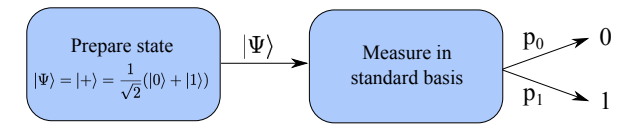
\includegraphics[width=1\linewidth]{Images/randomness.png}
    \caption{Genuine randomness from the preparation of a qubit in superposition}
    \label{fig:randomness}
\end{figure}
This simple example already tells us something about the power of quantum information: We could
build a machine that deterministically prepares the qubit $\ket{+}$, followed by a measurement in the
standard basis. Since $p_0=p_1=1/2$, this machine allows us to produce a perfect random number -
even though no randomness has been used inside our machine! In contrast, one can prove that no
classical deterministic machine can produce random numbers from scratch.

We saw how to measure a single qubit in the standard basis. The rule for computing probabilities
of measurement outcomes generalizes in a direct way to measuring n-qubit states. Indeed, consider
an n-qubit quantum state
\[
\ket{\Psi}=\sum_{x\in\{0,1\}^n} \alpha_x\ket{x}
\]
What happens when $\ket{\Psi}$ is measured in the standard basis $\ket{x}_x$? It turns out that the probability
of outcome x is given by $p_x = |\braket{x|\Psi}|^2=|\alpha_x|^2$, explaining again the need for normalization of
the vector $\ket{\Psi}$.

\subsubsection{Measuring a qubit in other bases}
Can we measure our qubit in any other basis? The answer to this is yes! Indeed this is another
feature that distinguishes quantum from classical, where the only basis around is the standard basis.
To find out how to analyze such a more general setting, let us first take a step back and consider
how we found the probabilities above. When measuring in the standard basis, the probabilities are given by the squared amplitudes when writing out the state in terms of the standard basis. When
measuring a qubit in a different orthonormal basis, given by vectors $\mathcal{G}=\{\ket{v},\ket{v^\perp}\}$, it is intuitive that we would have to express the qubit in the new basis. That is, we need to find amplitudes $\hat{\alpha}$ and $\hat{\beta}$ such that
\[
\ket{\psi}=\alpha\ket{0}+\beta\ket{1}=\hat{\alpha} \ket{v}+\hat{\beta}\ket{v^{\perp}}
\]
\begin{example}
    As an example, let consider again the qubit $\ket{+}=(1/\sqrt{2})(\ket{0}+\ket{1})$. Instead
of measuring it in the standard basis, let us now measure in the basis $H = \{\ket{+},\ket{-}\}$ given by
the two orthonormal vectors $\ket{+}$ and $\ket{-} = (1/\sqrt{2})(\ket{0}-\ket{1})$. Clearly, we can write the qubit as $1\ket{+}+0\ket{-}$. Thus the probability of obtaining measurement outcome “$\ket{+}$” is 1. We thus see
that the probabilities of measurement outcomes depends dramatically on the basis in which we
measure. 
\end{example}

\begin{example}
    Consider measuring an arbitrary qubit $\alpha\ket{0}+\beta\ket{1}$ in the basis $\{\ket{+},\ket{-}\}$. To
find out how to express the qubit in this other basis, it is convenient to determine how the basis
elements $\ket{0}$ and $\ket{1}$ look like in this basis. We find that
\[
\ket{0}=\frac{1}{2}[(\ket{0}+\ket{1})+(\ket{0}-\ket{1})]=\frac{1}{\sqrt{2}}(\ket{+}+\ket{-})
\]
\[
\ket{1}=\frac{1}{2}[(\ket{0}+\ket{1})-(\ket{0}-\ket{1})]=\frac{1}{\sqrt{2}}(\ket{+}-\ket{-})
\]
We thus have
\begin{align*}
\alpha\ket{0}+\beta\ket{1}&=\frac{1}{\sqrt{2}}[\alpha(\ket{+}+\ket{-})+\beta(\ket{+}-\ket{-})]\\
&=\frac{\alpha+\beta}{\sqrt{2}}\ket{+}+\frac{\alpha-\beta}{\sqrt{2}}\ket{-}
\end{align*}
This means that we obtain outcome "$\ket{+}$" with probability $|\alpha+\beta|^2/2$ and outcome "$\ket{-}$" with probability $|\alpha-\beta|^2/2$/
\end{example}

\begin{example}
    Consider the state $\ket{\Psi}=\ket{0}$. What are the probabilities  $p_0,p_1$ for measuring $\ket{\Psi}$ in the standard basis? What are the probability $p_{+},p_{-}$ for measuring $\ket{\Psi}$ in the Hadamard basis?
    For measuring in the standard basis the probabilities $p_0=1, p_1=0$. The probabilities in the Hadamard basis are $p_+=\frac{1}{2},p_-=\frac{1}{2}$.
\end{example}

Quite often we do not care about the entire probability distribution, but just the probability of one
specific outcome. Is there a more efficient way to find this probability than to rewrite the entire
state $\ket{\psi}$ in another basis? To investigate this, let us consider a single qubit
\[
\ket{\psi}=\alpha\ket{0}+\beta\ket{1}
\]
Remember that the elements of the standard basis are orthonormal. This means that
\[
(\ket{0})^{\dagger}\ket{0}=\begin{pmatrix} 1 & 0 \end{pmatrix}\begin{pmatrix} 1 \\ 0 \end{pmatrix} = 1,
\]
\[
(\ket{0})^{\dagger}\ket{1}=\begin{pmatrix} 1 & 0 \end{pmatrix}\begin{pmatrix} 0 \\ 1 \end{pmatrix} = 0
\]
Because the vectors are orthonormal, we could thus have found the desired probabilities by simply
computing the inner product between two vectors, as claimed above. Specifically, when given the qubit $\ket{\psi}=\alpha\ket{0}+\beta\ket{1}$ we obtain outcomes "$\ket{0}$" and "$\ket{1}$" with probabilities
\[
p_0=|\braket{0|\psi}|^2=\begin{vmatrix}\begin{pmatrix} 1 & 0 \end{pmatrix} \begin{pmatrix}\alpha \\ \beta \end{pmatrix}  \end{vmatrix}^2=|\alpha|^2
\]
\[
p_1=|\braket{1|\psi}|^2=\begin{vmatrix} \begin{pmatrix} 0 & 1 \end{pmatrix}\begin{pmatrix}\alpha \\ \beta \end{pmatrix}  \end{vmatrix}^2=|\beta|^2
\]

\begin{example}
    Suppose we measure $\ket{0}$ in the hadamard basis $\mathcal{H}$ (see above). The probabilities of observing outcomes "$\ket{+}$" and "$\ket{-}$" are given by
    \[
    p_+=|\braket{0|\psi}|^2=\begin{vmatrix}\begin{pmatrix} 1/\sqrt{2} & 1/\sqrt{2} \end{pmatrix} \begin{pmatrix}\alpha \\ \beta \end{pmatrix}  \end{vmatrix}^2=\frac{1}{2}
\]
\[
p_-=|\braket{1|\psi}|^2=\begin{vmatrix} \begin{pmatrix} 1/\sqrt{2} & 1/\sqrt{2} \end{pmatrix}\begin{pmatrix}\alpha \\ \beta \end{pmatrix}  \end{vmatrix}^2=\frac{1}{2}
\]
For multiple qubits, the rules for finding probabilities is analogous.
\end{example}

\begin{definition}
    Suppose that we measure a quantum state $\ket{\psi}$ in the orthonormal basis $\{\ket{b_j}\}_{j=1}^d$. The probability of observing outcome "$b_j$" can be found by computing
    \[
    p_j=|\braket{b_j|\psi}|^2
    \]
    The post-measurement state when obtaining outcome"$b_j$" is given by $\ket{b_j}$.
\end{definition}

Let us now consider some examples to gain intuition on measuring quantum systems in different
bases. First, let us have a look at a single qubit example.

\begin{example}
    Consider the qubit $\ket{\Psi}=\frac{1}{\sqrt{2}}(\ket{0}+\iota\ket{1})$, and measure the qubit in the $\{\ket{+},\ket{-}\}$ basis. the probabilities of obtaining "+" and "-" can be evaluated as follows:
    \begin{align*}
    p_+&=|\braket{\Psi|+}|^2=\begin{vmatrix} \dfrac{1}{2}(\bra{0}-\iota \bra{1})(\ket{0}+\ket{1})\end{vmatrix}^2\\
    &=\frac{1}{4}\begin{vmatrix} \braket{0|0}+\braket{0|1} - \iota\braket{1|0} - \iota \braket{1|1} \end{vmatrix}^2\\
    &=\frac{1}{4}|1-\iota|^2\\
    &=\frac{1}{4}(1-\iota)(1+\iota)=\frac{1}{2}
    \end{align*}
    \begin{align*}
    p_-&=|\braket{\Psi|-}|^2=\begin{vmatrix} \frac{1}{2}(\bra{0}-\iota \bra{1})(\ket{0}-\ket{1})\end{vmatrix}^2\\
    &=\frac{1}{4}\begin{vmatrix} \braket{0|0}+\braket{0|1} - \iota\braket{1|0} + \iota \braket{1|1} \end{vmatrix}^2\\
    &=\frac{1}{4}|1+\iota|^2\\
    &=\frac{1}{4}(1-\iota)(1+\iota)=\frac{1}{2}
    \end{align*}
\end{example}
This example shows that when the states involved have complex-valued amplitudes, one has to
take extra caution when evaluating the inner product: namely when taking the bra $\bra{\Psi}$, one should remember to alter the +/- sign whenever a complex number is involved (since the bra $\bra{\Psi}$ is the
conjugate transpose of the ket $\ket{\Psi}$). 

While we will generally talk about n-qubits, we can of course also consider a quantum system
comprised of three levels $\ket{0}$, $\ket{1}$, and $\ket{2}$, i.e. a qutrit. The rule for obtaining the probabilities of
measurement outcomes remains unchanged.

\begin{example}
    Consider a qutrit, which is a 3-dimensional quantum system represented by the vector
    \[
    \ket{v}=\frac{1}{\sqrt{2}}\begin{pmatrix} 1 \\ 0 \\ 0\end{pmatrix} + \frac{1}{\sqrt{2}}\begin{pmatrix} 0 \\ 1 \\ 0\end{pmatrix}\frac{1}{\sqrt{2}}\begin{pmatrix} 0 \\ 0 \\ 1\end{pmatrix}
    \]
    and measure in the basis $\mathcal{B}=\{\ket{b_1},\ket{b_2},\ket{b_3}\}$ where
    \[
    \ket{b_1}=\begin{pmatrix} 1 \\ 0 \\ 0 \end{pmatrix}, \quad \ket{b_2} = \frac{1}{\sqrt{2}}\begin{pmatrix} 0 \\ 1 \\ 1 \end{pmatrix}, \quad \frac{1}{\sqrt{2}}\begin{pmatrix} 0 \\ 1 \\ -1 \end{pmatrix} 
    \]
    The probabilities of obtaining each outcome can be calculated as follows:
    \[
    p_{b_1}=|\braket{b_1|v}|^2=\frac{1}{2}
    \]
    \[
    p_{b_2}=|\braket{b_2|v}|^2=\braket{b_2|v}\braket{v|b_2}=\frac{1}{2\sqrt{2}}(1+1)\frac{1}{2\sqrt{2}}(1+1)=\frac{1}{2}
    \]
    \[
    p_{b_3}=|\braket{b_3|v}|^2=\braket{b_3|v}\braket{v|b_3}|=\frac{1}{2\sqrt{2}}(1-1)\frac{1}{2\sqrt{2}}(1-1)=0
    \]
\end{example}

\subsubsection{Measurement Example I: Phase Estimation}
Now that we have discussed qubits in some detail, we can are prepared to
look more closesly at the measurement principle. Consider the quantum
state,
|\[
\ket{\psi}=\frac{1}{\sqrt{2}}\ket{0}+\frac{e^{\iota\theta}}{\sqrt{2}}\ket{1}
\]
If we were to measure this qubit in the standard basis, the outcome would
be $0$ with probability $1/2$ and $1$ with probability$ 1/2$. This measurement
tells us only about the norms of the state amplitudes. Is there any measurement that yields information about the phase, $\theta$?
To see if we can gather any phase information, let us consider a measurement in a basis other than the standard basis, namely
\[
\ket{+}=\frac{1}{\sqrt{2}}(\ket{0}+\ket{1}) \quad \text{and}\quad \ket{-}=\frac{1}{\sqrt{2}}(\ket{0}-\ket{1})
\]
What does $\ket{\phi}$ look like in this new basis? This can be expressed by first
writing,
\[
\ket{0}=\frac{1}{\sqrt{2}}(\ket{+}+\ket{-}) \quad \text{and} \quad \ket{-}=\frac{1}{\sqrt{2}}(\ket{0}-\ket{1})
\]
Now we are equipped to rewrite $\ket{\psi}$ in the $\{\ket{+}$, $\ket{-}\}$-basis,
\begin{align*}
\ket{\psi}&=\frac{1}{\sqrt{2}}\ket{0}+\frac{e^{\iota\theta}}{\sqrt{2}}\ket{1}\\
&=\frac{1}{2}(\ket{+}+\ket{-})+\frac{e^{\iota\theta}}{\sqrt{2}}(\ket{+}-\ket{-})\\
&=\frac{1+e^{\iota\theta}}{2}\ket{+}+\frac{1-e^{\iota\theta}}{2}\ket{-}
\end{align*}
Recalling the Euler relation, $e^{\iota theta}=\cos \theta+\iota\sin \theta$, we see that the probability
of measuring $\ket{+}$ is $\frac{1}{4}((1+\cos \theta)^2+\sin^2 \theta)=\cos^2 (\theta/2)$. A similar calculation reveals that the probability of measuring $\ket{-}$ is $\sin^2 (\theta/2)$ Measuring
in the ($ket{+},\ket{-}$)-basis therefore reveals some information about the phase $\theta$.
Later we shall show how to analyze the measurement of a qubit in a
general basis.

\subsubsection{Measurement example II: general Qubit Bases}
What is the result of measuring a general qubit state $\ket{\psi}=\alpha\ket{0}+\beta\ket{1}$, in
a general orthonormal basis $\ket{v}$, $\ket{v^{\perp}}$, where $\ket{v}=a\ket{0}+b\ket{1}$ and $\ket{v^{\perp}}=b^*\ket{0}-a^*\ket{1}$? You should also check that $\ket{v}$ and $\ket{v^{\perp}}$ are orthogonal by
showing that $\braket{v|v^{\perp}}=0$.

To answer this question, let us make use of our recently acquired braket notation. We first show that the states $\ket{v}$ and $\ket{v^{\perp}}$ are orthogonal, that is, that their inner product is zero:
\begin{align*}
\braket{v|v^{\perp}}&=(b^*\ket{0}-a^*\ket{1})^{\dagger}(a\ket{0}+b\ket{1})\\
&=(b\bra{0}-a\bra{1})^{\dagger}(a\ket{0}+b\ket{1})\\
&=ba\braket{0|0}-a^2\braket{1|0}+b^2\braket{0|1}-ab\braket{1|1}\\
&=ba-0+0-ab\\
&=0
\end{align*}

Here we have used the fact that $\braket{i|j}=\delta_{ij}$ .

Now, the probability of measuring the state $\ket{\psi}$ and getting $\ket{v}$ as a
result is,
\begin{align*}
p_{\psi}(v)&=|\braket{v|\psi}|^2\\
&=|(a^*\bra{0}+b^*\bra{1})(\alpha\ket{0}+\beta\ket{1})|^2\\
&=|a^*\alpha+b^*\beta|^2
\end{align*}
Similarly,
\begin{align*}
P_{\psi}(v^{\perp})&=|\braket{v^{\perp}|\psi}|^2\\
&=|(b\bra{0}-a\bra{1})(\alpha\ket{0}+\beta\ket{1})|^2\\
&=|b\alpha-\alpha\beta|^2
\end{align*}

\subsubsection{Expectation Values}
Physicists (but also computer scientists!) like to compute expectation values of measurement outcomes, as they provide an indication of the average behavior, if one was to perform a measurement many times (however we shall see later, that the measurement will perturb the state!). let us suppose that we measure a qubit $\ket{\Psi}$ in the standard basis $\{\ket{0},\ket{1}\}$. We will adopt the physics convention of labelling outcomes $\pm1$. This means that we associate the outcome "$\ket{0}$" with outcome $+1$, and outcome "$\ket{1}$" with outcome $-1$. The expectation value the outcome obtained when measuring $\ket{\psi}$ is then
\[
E=1|\braket{0|\psi}|^2-1\braket{1|\psi}|^2
\]
Note that since $|\braket{0|\psi}|^2=\braket{\psi|0}\braket{0|\psi}$, we have
\[
E=\bra{\psi}(\ket{0}\bra{0}-\ket{1}\bra{1})\ket{\psi}=\braket{\psi|Z|\psi}
\]
where $Z=\ket{0}\bra{0}-\ket{1}\bra{1}$.  As we shall see later, $Z$ is called the Pauli-Z matrix.

\subsection{Measuring Multiple Systems}
We saw how to measure some quantum state $\ket{\psi}$. let us now consider what happens if we measure the state of multiple qubits, where we think of measuring each qubit in a separate basis. To understand this, it is useful to realize that a basis for the join state space $\mathbb{C}_A^{d_A} \otimes \mathbb{C}_B^{d_B}$ can be obtained from bases for the individual state spaces $\mathbb{C}_A^{d_A}$ and $\mathbb{C}_B^{d_B}$. Specifically, if $\{\ket{b_j^A}\}_j$ is basis for $\mathbb{C}_A^{d_A}$ and $\{\ket{b_j^B}\}_j$ is a basis for the state space $\mathbb{C}_B^{d_B}$, then the set of vectors $\{\{\ket{b_j^A}\otimes \ket{b_k^B}\}_{j=1}^{d_A}\}_{k=1}^{d_B}$ gives a basis for $\mathbb{C}_A^{d_A}\otimes \mathbb{C}_B^{d_B}$.

\begin{example}
    Consider the basis $\{\ket{0}_A,\ket{1}_A\}$ for qubit A, and the basis \\$\{\ket{+}_B,\ket{-}_B\}$ for qubit B. A basis for the joint state AB is then given by \\
    $\{\ket{0}_A\ket{+}_B,\ket{0}_A\ket{-}_B,\ket{1}_A\ket{+}_B,\ket{1}_A\ket{-}_B\}$.
\end{example}

Let us not think how we might construct how we might construct some measurement for two quantum states from measurements of the individual ones. Suppose we measure particle A in the basis $\{\ket{b_j^A}\}_j$ and particle B in the basis $\{b_k^B\}_k$ when the joint state of both particles is given by $\ket{\psi}_{AB}$. What is the probability that we obtain outcome "$\ket{b_j^A}$" on A, and outcome "$\ket{b_k^B}$" on B? To find such joint probabilities, we first write down the joint basis fo quantum states A and B as above: $\{\{\ket{b_j^A}\ket{b_k^B}\}_j\}_k$. We can apply the usual rule to compute the probability as 
\[
p_{jk}=|\braket{b_j^A|\braket{b_k^B|\ket{\psi}_{AB}}}|^2
\]
\begin{example}
    Consider the two qubits in an EPR pair
    \[
    \ket{EPR}=\frac{1}{\sqrt{2}}(\ket{00}+\ket{11}
    \]
    and measure them both in the standard basis. The probabilities of obtaining outcomes 00, 01 ,10 and 11 are given by
    \[
    p_{00}=p_{11}=\frac{1}{2}
    \]
    \[
    p_{01}=p_{10}=0
    \]
\end{example}

\subsubsection{Partial Measurements}
Suppose we have a system consisting of two or more qubits and we only measure one of them. For
example, suppose the qubits are X and Y, and these qubits are in the state
\[
\ket{\psi}=\frac{1}{2}\ket{00}-\frac{\iota}{2}\ket{10}+\frac{1}{\sqrt{2}}\ket{11}
\]
We know what the distribution of measurement outcomes would be if we measured both qubits:
\[
Pr\text{[outcome is 00]} = \frac{1}{4} \quad Pr\text{[outcome is 01]}=0
\]
\[
Pr\text{[outcome is 10]}=\frac{1}{4} \quad pr\text{[outcome is 11]}=\frac{1}{2}
\]
The probability that a measurement of the first qubit, for instance, results in outcome $0$ should
therefore be $1/4+0 = 1/4$ and the probability of outcome $1$ should be $1/4+1/2 = 3/4$. Intuitively,
this should be the case regardless of whether or not the second qubit was actually measured. Indeed
this is the case.

However, what is different between the case where the second qubit is measured and the case
where it is not is the superposition of the system after the measurement (or measurements). If both
qubits are measured, the superposition will be one of $\ket{00},\ket{01},\ket{10}$, or $\ket{11}$, depending on the
measurement outcome. If only the first qubit is measured, however, this may not be the case.
I’ll explain how you determine the state of the system after the measurement of the first qubit
for the example above, and the method for a general case should be clear. We begin by considering
the possible outcome 0 for the measurement. We consider the state
\[
\ket{\psi}=\frac{1}{2}\ket{00}-\frac{\iota}{2}\ket{10}+\frac{1}{\sqrt{2}}\ket{11}
\]
and cross off all of the terms in the sum that are inconsistent with measuring a $0$ for the first qubit:
\[
\ket{\psi}=\frac{1}{2}\ket{00}
\]
which leaves
\[
\frac{1}{\ket{00}}
\]
The probability of measuring 0 is the norm-squared of this vector.
\[
Pr\text{[measurement outcomes is 0]}=|\\frac{1}{2}\ket{00}\|=\frac{1}{4}
\]
and the state of the two qubits after the measurement conditioned on the measurement outcome being 0 is the vector itself renormalized:
\[
\frac{\frac{1}{2}\ket{00}}{\|\frac{1}{2}\ket{00}\|}=\ket{00}
\]
The possible measurement outcome 1 is handled similarly. we cross off the terms is inconsistent with measuring a 1 which leaves
\[
-\frac{\iota}{2}\ket{10}+\frac{1}{\sqrt{2}}\ket{11}
\]
The probability of measuring a 1 is then the norm-squared of this vector,
\[
Pr\text{measurement outcome is 1]}=\|-\frac{\iota}{2}\ket{10}+\frac{1}{\sqrt{2}}\ket{11}\|^2=|-\frac{\iota}{2}|^2+|\frac{1}{\sqrt{2}}|^2=\frac{3}{4}
\]
and conditioned on measuring a 1 is then the norm-squared of this vector
\[
\frac{-\frac{\iota}{2}\ket{10}+\frac{1}{\sqrt{2}}\ket{11}}{\|-\frac{\iota}{2}\ket{10}+\frac{1}{\sqrt{2}}\ket{11}\|}=-\frac{\iota}{\sqrt{3}}\ket{10}+\sqrt{\frac{2}{3}}\ket{11}
\]
A completely equivalent way of performing this calculation is to begin by writing
\[
\ket{\psi}=\ket{0}\ket{\phi_0}+\ket{1}\ket{\phi_1}
\]
for some choice of $\ket{\phi_0}$ and $\ket{\phi_1}$. (There will always be a unique choice for each that works.) in this case we have
\[
\ket{\psi}=\ket{0}\left(\frac{1}{2}\ket{0}\right)+\ket{1}\left(-\frac{\iota}{2}\ket{0}+\frac{1}{\sqrt{2}}\ket{1}\right)
\]
so $\ket{\phi_0}=\frac{1}{2}\ket{0}$ and $\ket{\phi_1}=-\frac{\iota}{2}\ket{0}+\frac{1}{\sqrt{2}}\ket{1}$. The probabilities for the two measurement outcomes are as follows:
\[
Pr\text{[outcome is 0]}=\|\ket{\phi_0}\|^2=|\frac{1}{2}|^2=\frac{1}{4}
\]
\[
Pr\text{[outcome is 1]}=\|\ket{\phi_1}\|^2=|-\frac{\iota}{2}|^2+|\frac{1}{\sqrt{2}}|^2=\frac{3}{4}
\]
Conditioned on the measurement outcome, the state of the two qubits is as follows:
\[
\text{measurement outcome is 0}\implies \text{state becomes} \frac{1}{\|\ket{\phi_0}\|}\ket{0}\ket{\phi_0}=\ket{00}
\]
\[
\text{measurement outcome is 1} \implies \text{state becomes}\frac{1}{\|\ket{\phi_1}}\ket{1}\ket{\phi_1}=\frac{-\iota}{\sqrt{3}}\ket{10}+\sqrt{\frac{2}{3}}\ket{11}
\]
The same method works for more than 2 qubits as well.

\begin{example}
    Suppose 3 qubits are in the superposition
    \[\ket{\psi}=\frac{1}{2}\ket{000}+\frac{1}{2}\ket{100}+\frac{1}{2}\ket{101}-\frac{1}{2}\ket{111}\]
    and the third qubit is measured. What are the probabilities of the two possible measurement outcomes and what are the resulting superpositions of the three qubits for each case?
    To determine the answer we ewrite,
    \[
    \ket{\psi}=\left(\frac{1}{2}\ket{00}+\frac{1}{2}\ket{10}\right)\ket{0}+\left(\frac{1}{2}\ket{10}-\frac{1}{2}\ket{11}\right)\ket{1}
    \]
    The probability that the measurement outcome is 0 is
    \[
    \|\frac{1}{2}\ket{00}+\frac{1}{2}\ket{10}\|^2=\frac{1}{2}
    \]
    and in this case the resulting superposition is 
    \[
    \sqrt{2}\left(\frac{1}{2}\ket{00}+\frac{1}{2}\ket{10}\right)\ket{0}=\frac{1}{\sqrt{2}}\ket{000}+\frac{1}{\sqrt{2}}\ket{100}
    \]
    The probability that the measurement outcome is 1 is
    \[
    \|\frac{1}{2}\ket{10}-\frac{1}{2}\ket{11}\|^2=\frac{1}{2}
    \]
    and in this case the resulting superposition is
    \[
    \sqrt{2}\left(\frac{1}{2}\ket{10}-\frac{1}{2}\ket{11}\right)\ket{1}=\frac{1}{\sqrt{2}}\ket{101}-\frac{1}{\sqrt{2}}\ket{111}
    \]
\end{example}
\section{The Stern-Gerlach Experiment}
The concepts of superposition and entanglement are counter-intuitive to our daily experiences. The following experiment proves that the nature truly operates in this peculiar manner. It provides the proof for existence of qubits in Nature. thus, showing that the relalization of large-scale quantum computers will be experimentally feasible.

The qubit is a fundamental element for quantum computation and quantum information. An early experiment indicating the qubit structured was performed by Stern in 1921 and Gerlach in 1922 in frankfurt. In the original Stern-Gerlach Experiment, hot atoms were 'beamed' from an oven through a magnetic filed which caused the atoms to be deflected, and then the position of each atom was recorded. The original experiment was done with silver atoms, which have a complicated structure that obscures the effects we are discussing. What we describe below actually follows a 1927 experiment done using hydrogen atoms. The same basic effect is observed, but with hydrogen atoms the discussion is easier to follow. Keep in mind, though, that this privilege wasn't available to people in the early 1920s, and they have to be very ingenious to think up explanations for the more complicated effects they observed.

Hydrogen atoms contain a proton and an orbiting electron. you can think of this electron as a little 'electric current' around the proton. This electric current causes the atom to have a magnetic filed; each atom has what physicists call a `magnetic dipole moment'. As a result each atom behaves like a little bar magnet with an axis corresponding to the axis the electron is spinning around. throwing little bar magnet is through a magnetic filed causes the magnets to be deflected by the field, and we expect to see a similar deflection of atoms in the Stern-Gerlach experiment.

How the atom is deflected depends upon both the atom's magnetic dipole moment - the axis the electron is spinning around and the magnetic filed generated by the Stern-Gerlach device. We won't go through the details, but suffice to say that by constructing the Stern-Gerlach device appropriately, we can cause the atom to be deflected by an amount that depends upon the $\hat{z}$ component of the atom's magnetic dipole moment, where $\hat{z}$ is some fixed external axis.

Two major surprises emerge when this experiment is performed. First, since the hot atoms exiting the oven would naturally be expected to have their dipoles oriented randomly in every direction, it would follow that there would be a continuous distribution of atoms seen at all angles exiting from the Stern-gerlach device. Instead, what is seen is atoms emerging from a discrete set of angles. Physicists were able to explain this by assuming that the magnetic dipole moment of atoms is quantized, that is, comes in discrete multiples of some fundamental amount.

This observation of quantization in the Stern-Gerlach experiment was surprising to physicists of the 1920s, but not completely astonishing because evidence of quantization effects in other systems was becoming widespread at that time. What was truly surprising was the number of peaks seen in the experiment. The hydrogen atoms being used were such that they should have zero magnetic dipole moment. Classically, this is surprising in itself, since it corresponds to no orbital motion of the electron, but based on what was known of quantum mechanics at that time was an acceptable notion. Since the hydrogen atoms would therefore have zero magnetic moment, it was expected that only one beam of atoms would be seen, and this beam would not be deflected by the magnetic field. instead, two beams were seen, one deflected up by the magnetic field and the other deflected down.

This puzzling doubling was explained after considerable effort by positioning that the electron in the hydrogen atoms has associated with it a quantity called spin. This spin is not in any way associated to the usual rotational motion of the electron around the proton; it is an entirely new quantity associated with with an electron. The great physicist Heisenberg labeled the idea `brave' at the time it was suggested, and it is a brave idea, since it introduces an essentially new physical quantity into Nature. The spin of the electron is posited to make an extra contribution to the magnetic dipole moment of a hydrogen atom, in addition to the contribution due to the rotational motion of the electron.
\begin{figure}
    \centering
    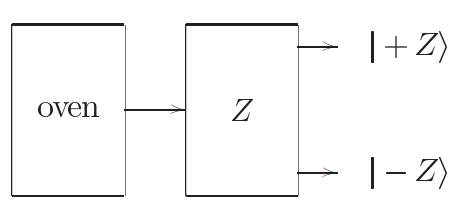
\includegraphics[width=0.5\linewidth]{Images/stern-gerlach.png}
    \caption{Abstract schematic of Stern-Gerlach experiment. Hot hydrogen atoms are beamed from an oven through a magnetic field, causing a deflection either up $(\ket{+Z})$ or down $(\ket{-Z})$}
    \label{fig:abs-sgexp}
\end{figure}
What is the proper description of the spin of the electron? As a first guess, we might hypothesize that the spin is specified by a single bit, telling the hydrogen atom to go up or down. Additional experimental results provide further useful information to determine if this guess needs refinement or replacement. Let's represent the original Stern-Gerlach apparatus as shown in the figure \ref{fig:3stage-sgexp}. Its outputs are two beams of atoms, which we shall called $\ket{+Z}$ and $\ket{-Z}$. (We're using suggestive notation which looks quantum mechanics, but of course you're free to use whatever notation you prefer). Now suppose we cascade two Stern-Gerlach apparatus together, as shown in the figure \ref{fig:casc-sgexp}. We arrange it so that the second apparatus is tipped sideways, so the magnetic field deflects the atoms along the $\hat{x}$ axis. In our thought-experiment we'll block off the $\ket{-Z}$ output from the first Stern-Gerlach apparatus, while the $\ket{+Z}$ output is sent through a second apparatus oriented along the $\hat{x}$ axis. A detector is placed at the final output to measure the distribution of atoms along the $\hat{x}$ axis.

A classical magnetic dipole pointed in the $+\hat{z}$ direction has no net magnetic moment in the $\hat{x}$ direction, so we might expect that the final output would have one central peak. However, experimentally it is observed that there are two peaks of equal intensity! So perhaps these atoms are peculiar, and have definite magnetic moments along each axis, independently. That is, maybe each atom passing through the second apparatus can be described as being in a state we might write as $\ket{+Z}\ket{+X}$ or $\ket{+Z}\ket{-X}$, to indicate the two values for spin that might be observed. 
\begin{figure}
    \centering
    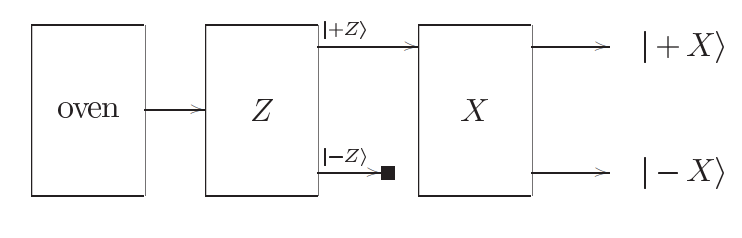
\includegraphics[width=0.65\linewidth]{Images/casca_sgexp.png}
    \caption{Cascaded Stern-gerlach Experiment}
    \label{fig:casc-sgexp}
\end{figure}
\begin{figure}
    \centering
    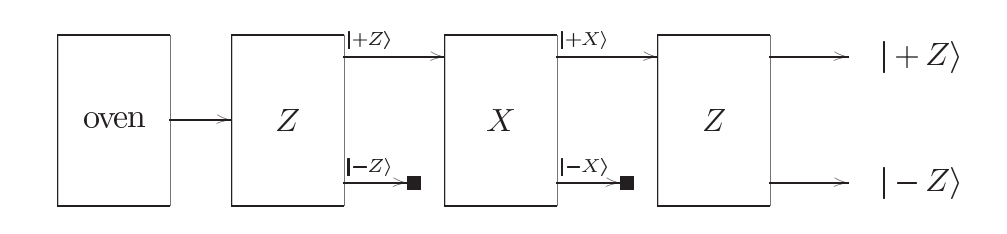
\includegraphics[width=0.75\linewidth]{Images/3stage-sgexp.png}
    \caption{Three stage cascaded Stern-Gerlach measurements}
    \label{fig:3stage-sgexp}
\end{figure}
Another experiment, shown in figure \ref{fig:casc-sgexp}, can test this hypothesis by sending one beam of the previous output through a second $\hat{z}$ oriented Stern-Gerlach apparatus. If the atoms had retained their $\ket{+Z}$ orientation, then the output would be expected to have only one peak at the $\ket{+Z}$ output. However, again tow beams are observed at the final output, of equal intensity. Thus, the conclusion would seem to be that contrary to classical expectations, a $\ket{+Z}$ state consists of equal portions of $\ket{+Z}$ and $\ket{-X}$ states, and a $\ket{+X}$ state consists of equal portions of $\ket{+Z}$ and $\ket{-Z}$ states. Similar conclusions can be reached if the Stern-Gerlach apparatus is aligned along some other axis like the $\hat{y}$ axis.

The qubit model provides a simple explanation of this experimentally observed behavior. Let $\ket{0}$ and $\ket{1}$ be the states of a qubit, and make the assignments.
\begin{align*}
    \ket{+Z} &\leftarrow \ket{0}\\
    \ket{-Z} &\leftarrow \ket{1}\\
    \ket{+X} &\leftarrow (\ket{0}+\ket{1})/\sqrt{2}\\
    \ket{-X} &\leftarrow (\ket{0}- \ket{1})/\sqrt{2}
\end{align*}
then the results of the cascaded Stern-Gerlach experiment can be explained by assuming that the $\hat{z}$ Stern-Gerlach apparatus measures the spin (that is, the qubit) in the computational $\ket{0},\ket{1}$, and the $\hat{x}$ Stern-Gerlach apparatus measures the spin with respect to the basis $(\ket{0}+\ket{1})/\sqrt{2}, (\ket{0}-\ket{1})/\sqrt{2}$. For example, in the cascaded $\hat{z}-\hat{x}-\hat{z}$ experiment, if we assume that the spin are in the state $\ket{+Z}=\ket{0}=(\ket{+X}+\ket{-X})/\sqrt{2}$ after exiting the first Stern-gerlach experiment, then the probability for obtaining $\ket{+X}$ out of the second apparatus is $1/2$, and the probability for $\ket{-X}$ is 1/2. Similarly, the probability for obtaining $\ket{+Z}$ out of the third apparatus is $1/2$. A qubit model thus properly predicts results from this type of cascaded Stern-Gerlach experiment.

This example demonstrates how qubits could be a believable way of modelling systems in Nature. Of course it doesn't establish beyond all doubt that the qubit model is the correct way of understanding electron spin - far more experimental corroboration is required. nevertheless, because of many experiments like these, we now believe that the qubit model (and generalizations of it to higher dimensions; quantum mechanics in other words) is capable of describing every physical system.

\section{Qiskit Examples}
In this section we present some examples of Qiskit implementations of the concepts introduced in this lesson.

\subsection{Vector and Matrices in Python}
Qiskit uses the Python programming language, so before discussing Qiskit specifically it may be helpful to very briefly discuss matrix and vector computations in Python. In Python, matrix and vector computations can be performed using the  array  class from the  NumPy  library (which includes many additional components for numerical computation).

Here is an example of a code cell that defines two vectors,  ket0  and  ket1, corresponding to the qubit state vectors $\ket{0}$ and $\ket{1}$ and displays their average.
\begin{lstlisting}[language=Python]
from numpy import array

ket0 = array([1, 0])
ket1 = array([0, 1])

display(ket0 / 2 + ket1 / 2)
\end{lstlisting}
Output:
\begin{lstlisting}
array([0.5, 0.5])
\end{lstlisting}
It is not actually necessary to explicitly use the  display  command to see the result of this computation. We may instead simply write the expression of interest as the last line of the code cell, and it will be returned as its output:
\begin{lstlisting}[language=Python]
ket0 / 2 + ket1 / 2
\end{lstlisting}
Output:
\begin{lstlisting}
array([0.5, 0.5])
\end{lstlisting}

This code cell also illustrates that running code cells sequentially on a given page of this textbook has a cumulative effect, so it is not necessary to reload the  array  class or define ket0  and  ket1  again. Reloading the page or switching to another page will, however, reset everything to its initial state.

As a general guideline, code cells within each subsection of this course are intended to be run sequentially. So, if running a code cell generates an error, be sure to first run all previous code cells within the subsection in which that code cell appears.

We can also use  array  to create matrices that represent operations.
\begin{lstlisting}[language=Python]
M1 = array([[1, 1], [0, 0]])
M2 = array([[1, 1], [1, 0]])

M1 / 2 + M2 / 2
\end{lstlisting}
Output:
\begin{lstlisting}
array([[1. , 1. ],
       [0.5, 0. ]])
\end{lstlisting}
Matrix multiplication (including matrix-vector multiplication as a special case) can be performed using the  matmul  function from  NumPy  :
\begin{lstlisting}[language=Python]
from numpy import matmul

display(matmul(M1, ket1))
display(matmul(M1, M2))
display(matmul(M2, M1))
\end{lstlisting}
Output:
\begin{lstlisting}
array([1, 0])
array([[2, 1],
       [0, 0]])
array([[1, 1],
       [1, 1]])
\end{lstlisting}

\subsection{States, measurements and operations}
Qiskit includes several classes that allow for states, measurements, and operations to be easily created and manipulated — so starting from scratch and programming everything that is needed to simulate quantum states, measurements, and operations in Python is not required. Some examples to get started are included below.

\subsubsection{Defining and displaying state vectors}

Qiskit's  Statevector  class provides functionality for defining and manipulating quantum state vectors. The following code cell imports the  Statevector  class and defines a few vectors using it. (Note that we need the  sqrt  function from the  NumPy  library to compute the square roots for the vector  u .)
\begin{lstlisting}[language=Python]
from qiskit.quantum_info import Statevector
from numpy import sqrt

u = Statevector([1 / sqrt(2), 1 / sqrt(2)])
v = Statevector([(1 + 2.0j) / 3, -2 / 3])
w = Statevector([1 / 3, 2 / 3])

print("State vectors u, v, and w have been defined.")
\end{lstlisting}
Output:
\begin{lstlisting}
State vectors u, v, and w have been defined.
\end{lstlisting}

The  Statevector  class provides a  draw  method for displaying state vectors, including latex  and  text  options for different visualizations, as this code cell demonstrates:

\begin{lstlisting}[language=Python]
display(u.draw("latex"))
display(v.draw("text"))
\end{lstlisting}
Output:
\[
\frac{\sqrt{2}}{2}\ket{0}+\frac{\sqrt{2}}{2}\ket{1}
\]
\[
[ 0.33333333+0.66666667j,-0.66666667+0.j ]
\]
The  Statevector  class also includes the  is\_valid  method, which checks to see if a given vector is a valid quantum state vector (i.e., that it has Euclidean norm equal to 1):
\begin{lstlisting}[language=Python]
display(u.is_valid())
display(w.is_valid())
\end{lstlisting}
Output:
\begin{lstlisting}
True

False
\end{lstlisting}
\subsubsection{Simulating Measurements using Statevector}
Next we will see one way that measurements of quantum states can be simulated in Qiskit, using the  measure  method from the  Statevector  class.

First, we create a qubit state vector  v  and then display it.
\begin{lstlisting}[language=Python]
v = Statevector([(1 + 2.0j) / 3, -2 / 3])
v.draw("latex")
\end{lstlisting}
Output:
\[
\left(\frac{1}{3}+\frac{2\iota}{3}\right)\ket{0}-\frac{2}{3}\ket{1}
\]
Next, running the  measure  method simulates a standard basis measurement. It returns the result of that measurement, plus the new quantum state of our system after that measurement
\begin{lstlisting}[language=Python]
v.measure()
\end{lstlisting}
Output:
\begin{lstlisting}
('1',
 Statevector([ 0.+0.j, -1.+0.j],
             dims=(2,)))
\end{lstlisting}
Measurement outcomes are probabilistic, so the same method can return different results. Try running the cell a few times to see this. 

For the particular example of the vector v, defined above, the measure method defines the quantum state vector after the measurement takes place to be
\[
\frac{1+2\iota}{\sqrt{5}}\ket{0}
\]
(rather than $\ket{0}$) or
\[
-\ket{1}
\]
(rather than $\ket{1}$), depending on the measurement outcome. In bot cases, the alternatives are, in fact, equivalent - they are said to differ by a global phase because one is equal to the other multiplied by a complex number on the unit circle. This issue is discussed in greater detail in the next chapter.

As an aside, Statevector will throw an error if the measure method is applied to an invalid quantum state vector. Feel free to give it a try if you are interested in seeing what an error looks like.

State vector also comes with a sample\_counts method that allows for the simulation of any number of measurements on the system. For example, the following cell shows the outcome of measuring the vector v 1000 times, which (with high probability) results in the outcome 0 approximately 5 out of every 9 times (or about 556 of the 1000 trials) and the outcome 1 approximately 4 out of every 9 times (or about 444 out of the 100 trials). The cell also demonstrates the plot\_histogram function for visualizing the results.

\begin{lstlisting}[language=Python]
from qiskit.visualization import plot_histogram

statistics = v.sample_counts(1000)
display(statistics)
plot_histogram(statistics)
\end{lstlisting}
Output:
\begin{lstlisting}
{np.str_('0'): np.int64(568), np.str_('1'): np.int64(432)}
\end{lstlisting}

\begin{figure}[ht]
    \centering
    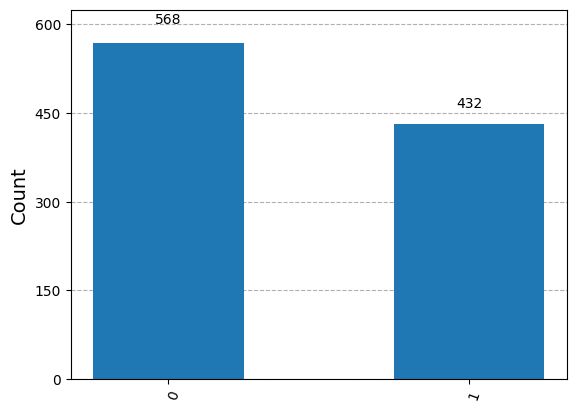
\includegraphics[width=0.75\textwidth]{Images/histogram_exp.png}
    \caption{Histogram of measurement outcomes}
\end{figure}

Running the cell multiple times and trying different numbers of samples in place of 1000 may be helpful for developing some intuition for how the number of trials influences the estimated probabilities.

\subsubsection{Performing operations with Operator and Statevector}
Unitary operations can be defined and performed on state vectors in Qiskit using the operator class, as in the example that follows:

\begin{lstlisting}[language=Python]
from qiskit.quantum_info import Operator

X = Operator([[0, 1], [1, 0]])
Y = Operator([[0, -1.0j], [1.0j, 0]])
Z = Operator([[1, 0], [0, -1]])
H = Operator([[1 / sqrt(2), 1 / sqrt(2)], [1 / sqrt(2), -1 / sqrt(2)]])
S = Operator([[1, 0], [0, 1.0j]])
T = Operator([[1, 0], [0, (1 + 1.0j) / sqrt(2)]])

v = Statevector([1, 0])

v = v.evolve(H)
v = v.evolve(T)
v = v.evolve(H)
v = v.evolve(T)
v = v.evolve(Z)

v.draw("text")
\end{lstlisting}
Output:
\begin{lstlisting}
[ 0.85355339+0.35355339j,-0.35355339+0.14644661j]
\end{lstlisting}

\subsubsection{Looking ahead toward Quantum Circuits}
Quantum circuits won't be formally introduced until the next few chapters, but we can nevertheless experiment with composing qubit unitary operations using Qiskit's QuantumCircuit class. In particular, we may define a quantum circuit (which in this case will simply be a sequence of unitary operations performed on a single qubit)

\begin{lstlisting}[language=Python]
from qiskit import QuantumCircuit

circuit = QuantumCircuit(1)

circuit.h(0)
circuit.t(0)
circuit.h(0)
circuit.t(0)
circuit.z(0)

circuit.draw()
\end{lstlisting}
Output:
\begin{figure}[ht]
    \centering
    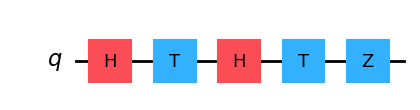
\includegraphics[width=0.75\textwidth]{Images/circuit_exp.png}
    \caption{Quantum Circuit}
\end{figure}
The operations are applied sequentially, starting on the left and ending on the right in the figure. Let us first initialize a starting quantum state vector and then evolve that state according to the sequence of operations.

\begin{lstlisting}[language=Python]
ket0 = Statevector([1, 0])
v = ket0.evolve(circuit)
v.draw("text")
\end{lstlisting}
Output:
\begin{lstlisting}
[ 0.85355339+0.35355339j,-0.35355339+0.14644661j]
\end{lstlisting}

Finally, let's simulate the result of running this experiment (i.e., preparing the state $\ket{0}$, applying the sequence of operations represented by the circuit, and measuring 4000 times.

\begin{lstlisting}[language=Python]
statistics = v.sample_counts(4000)
plot_histogram(statistics)
\end{lstlisting}
Output:
\begin{figure}[ht]
    \centering
    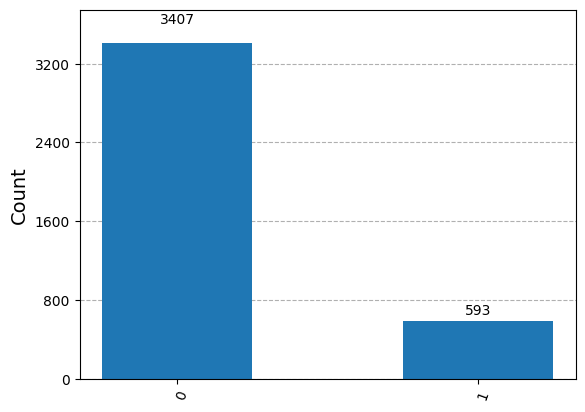
\includegraphics[width=0.75\textwidth]{Images/histogram_exp2.png}
    \caption{Histogram of measurement outcomes}
\end{figure}
In the previous lesson, we learned about Qiskit's Statevector and Operator classes, and used them to simulate quantum systems. In this section, we'll use them to explore the behavior of multiple systems. We'll start by importing these classes, as well as the square root function from NumPy .

\begin{lstlisting}[language=Python]
from qiskit.quantum_info import Statevector, Operator
from numpy import sqrt
\end{lstlisting}

\subsubsection{Tensor products}
The Statevector class has a tensor method which returns the tensor product of itself and another Statevector .

For example, below we create two state vectors representing $\ket{0}$ and $\ket{1}$, and use the tensor method to create a new vector, $\ket{0}\otimes \ket{1}$.
\begin{lstlisting}[language=Python]
zero, one = Statevector.from_label("0"), Statevector.from_label("1")
zero.tensor(one).draw("latex")
\end{lstlisting}
Output:
\[
\ket{01}
\]
In another example below, we create state vectors representing the 
$\ket{+}$ and $\frac{1}{\sqrt{2}}(\ket{0}+\iota\ket{1})$ states, and combine them to create a new state vector. We'll assign this new vector to the variable psi.
\begin{lstlisting}[language=Python]
plus = Statevector.from_label("+")
i_state = Statevector([1 / sqrt(2), 1j / sqrt(2)])
psi = plus.tensor(i_state)

psi.draw("latex")
\end{lstlisting}
Output:
\[
\frac{1}{2}\ket{00}+\frac{\iota}{2}\ket{01}+\frac{1}{2}\ket{10}+\frac{\iota}{2}\ket{11}
\]
The Operator class also has a tensor method. In the example below, we create the X and I gates and display their tensor product.
\begin{lstlisting}[language=Python]
X = Operator([[0, 1], [1, 0]])
I = Operator([[1, 0], [0, 1]])

X.tensor(I)
\end{lstlisting}
Output:
\begin{lstlisting}
Operator([[0.+0.j, 0.+0.j, 1.+0.j, 0.+0.j],
          [0.+0.j, 0.+0.j, 0.+0.j, 1.+0.j],
          [1.+0.j, 0.+0.j, 0.+0.j, 0.+0.j],
          [0.+0.j, 1.+0.j, 0.+0.j, 0.+0.j]],
         input_dims=(2, 2), output_dims=(2, 2))
\end{lstlisting}
We can then treat these compound states and operations as we did single systems in the previous lesson. For example, in the cell below we calculate $(I\otimes X)\ket{\psi}$ for the state psi we defined above. (The operator shown tensors matrices together.)
\begin{lstlisting}[language=Python]
psi.evolve(I ^ X).draw("latex")
\end{lstlisting}
\[
\frac{\iota}{2}\ket{00}+\frac{1}{2}\ket{01}+\frac{\iota}{2}\ket{10}+\frac{1}{2}\ket{11}
\]
Below, we create a CX operator and calculate $CX\ket{\psi}$.
\begin{lstlisting}[language=Python]
CX = Operator(
    [
        [1, 0, 0, 0],
        [0, 1, 0, 0],
        [0, 0, 0, 1],
        [0, 0, 1, 0],
    ]
)

psi.evolve(CX).draw("latex")
\end{lstlisting}
\[
\frac{1}{2}\ket{00}+\frac{\iota}{2}\ket{01}+\frac{\iota}{2}\ket{10}+\frac{1}{2}\ket{11}
\]

\subsection{Partial measurements}
In the previous page, we used the measure method to simulate a measurement of the quantum state vector. This method returns two items: the simulated measurement result, and the new Statevector given this measurement.

By default, measure measures all qubits in the state vector, but we can provide a list of integers to only measure the qubits at those indices. To demonstrate, the cell below creates the state $W=(\ket{001}+\ket{001}+\ket{010}+\ket{100})$
(Note that Qiskit is primarily designed for use with qubit-based quantum computers. As such, Statevector will try to interpret any vector with elements as a system of n qubits. You can override this by passing a dims argument to the constructor. For example, dims=(4,2) would tell Qiskit the system has one four-level system, and one two-level system (qubit).)
\begin{lstlisting}[language=Python]
W = Statevector([0, 1, 1, 0, 1, 0, 0, 0] / sqrt(3))
W.draw("latex")
\end{lstlisting}
\[
\frac{\sqrt{3}}{3}\ket{001}+\frac{\sqrt{3}}{3}\ket{010}+\frac{\sqrt{3}}{3}\ket{100}
\]
The cell below simulates a measurement on the rightmost qubit (which has index 0). The other two qubits are not measured.
\begin{lstlisting}[language=Python]
result, new_sv = W.measure([0])  # measure qubit 0
print(f"Measured: {result}\nState after measurement:")
new_sv.draw("latex")
\end{lstlisting}
Output:
\begin{lstlisting}
Measured: 1
State after measurement:
\end{lstlisting}
\[
\ket{001}
\]
Try running the cell a few times to see different results. Notice that measuring a 1 means that we know both the other qubits are 
$\ket{0}$, but measuring a 0 means the remaining two qubits are in the state $\frac{1}{\sqrt{2}}(\ket{01}+\ket{10})$.


\chapterreferences
